%% groupaffect4_devkit.tex  (arXiv devkit / technical report)
%% Title: GroupAffect-4 Devkit
%%
%% Compile:
%%   pdflatex groupaffect4_devkit
%%   bibtex   groupaffect4_devkit
%%   pdflatex groupaffect4_devkit
%%   pdflatex groupaffect4_devkit

\documentclass[sigconf,nonacm]{acmart}

\usepackage{booktabs}
\usepackage{multirow}
\usepackage{enumitem}
\usepackage{amsmath}
\usepackage{xcolor}
\usepackage{graphicx}
\usepackage{microtype}
\usepackage{listings}
\lstset{
  basicstyle=\ttfamily\scriptsize,
  breaklines=true,
  breakatwhitespace=false,
  columns=flexible,
  keepspaces=true,
  showstringspaces=false,
  frame=none,
  xleftmargin=0pt,
  xrightmargin=0pt
}
\usepackage{balance}  % even final columns
\usepackage{caption}  % caption* support
% natbib is loaded by acmart; do not reload
\usepackage{tikz}
\usetikzlibrary{arrows.meta, positioning, shapes.geometric, fit, backgrounds}

\acmConference[arXiv]{GroupAffect-4 Devkit Technical Report}{2026}{}
\acmYear{2026}
\copyrightyear{2026}
\setcopyright{none}

\settopmatter{printacmref=false}
\renewcommand\footnotetextcopyrightpermission[1]{}
\pagestyle{plain}

% ── Macros ─────────────────────────────────────────────────────────────────
\newcommand{\bfibold}{\textsc{bfi}}
\newcommand{\F}[1]{\mbox{F1}_{#1}}
\definecolor{bestcol}{HTML}{1a6e1a}
\newcommand{\best}[1]{\textbf{\textcolor{bestcol}{#1}}}

\renewcommand{\arraystretch}{1.1}       % comfortable vertical table row spacing
\hyphenation{Match-N-Min-gle Neuro-Kit2}% allow breaks in proper-noun compounds

% ── Title ──────────────────────────────────────────────────────────────────
\title{GroupAffect-4 Devkit: Target Construction, Augmentation, Preprocessing,
       and Temporal Modeling for Physiological Affect Sensing}

\author{Meisam Jamshidi Seikavandi}
\affiliation{%
  \institution{CogniSense Lab, GN Hearing}
  \city{Copenhagen}
  \country{Denmark}}
\email{mjse@gn.com}

\begin{document}
\setlength{\emergencystretch}{40pt}  % prevent overfull hboxes

% ═══════════════════════════════════════════════════════════════════════════
\begin{abstract}
\noindent\textit{Who is this for?}
Researchers who want to study physiological affect recognition in real
four-person collaborative groups and need a reproducible modelling starting
point, or who want to extend, benchmark against, or cite the GroupAffect-4
dataset.
All code and data are publicly released; see \S\ref{sec:data_access} and
Appendix~\ref{sec:appendix_repro} for access instructions and
step-by-step reproduction.

GroupAffect-4 is a small but dense multimodal dataset for studying affect in
four-person collaborative interaction: 39 participants across 10 sessions,
wearable physiology and eye tracking, Big Five personality, post-task
Valence--Arousal--Dominance (VAD) self-reports, and post-block questionnaires.
This manuscript is a modelling devkit for the dataset rather than a single
narrow benchmark paper.
It defines the target-construction pipeline, evaluation regimes, baseline
models, label-augmentation variants, preprocessing/windowing ablations, ordinal
training path, and temporal self-supervised modelling recipes needed to use
GroupAffect-4 reproducibly.
The central empirical constraint is label scarcity: 292 labelled 15-second
windows, with only 103 windows in the canonical train split, must supervise
thousands of unlabelled physiological windows.
Under this constraint, balanced midpoint-tertile labels and per-dimension class
weights establish an honest three-class benchmark (RBF-SVM $0.495$ macro-F1)
and a parallel ordinal baseline (MAE\,$=$\,1.474, Spearman\,$=$\,0.324).
Personality-weighted augmentation using BFI-44 cosine similarity as a
cross-person trust weight reaches $0.526$ macro-F1 in the known-team setting,
but session-isolated LOGO evaluation shows that this gain does not transfer to
entirely unseen groups ($0.262$ vs.\ $0.266$ no-aug).
Preprocessing matters as much as modelling: smoothing only EDA and PPG while
preserving gaze, pupil, and IMU features improves all three VAD dimensions
($V{=}0.600$, $A{=}0.624$, $D{=}0.436$).
Reprocessing gaze/pupil features from raw sequences with improved NaN handling
changes the Dominance trade-off (up to $D{=}0.492$ in unsmoothed all-modality
v2); under canonical centred-smoothing comparisons, the confirmed
single-pipeline best remains $0.553$, and a per-dimension upper bound reaches
$0.561$.
Finally, temporal Conv1D/BiGRU encoders and SimCLR/MSM pre-training define a
separate sequence-modelling track, where per-dimension SimCLR configurations
can exceed SVM+AP1 on Arousal and Dominance.
We close with recommended devkit recipes and a claim-status map for extracting
future focused papers on label augmentation, preprocessing, and temporal
modelling.
\end{abstract}

\keywords{physiological affect sensing, label scarcity, VAD prediction,
Gaussian Process augmentation, Big Five personality, label augmentation,
ordinal labels, wearable sensing}

% ═══════════════════════════════════════════════════════════════════════════
\maketitle

\section*{Version, Scope, and How to Read This Document}
\label{sec:version_scope}

\noindent\textbf{Purpose.}
This arXiv report is the stable technical reference for the GroupAffect-4
dataset and modelling toolkit.
It is \emph{not} a narrow benchmark paper making a single head-to-head claim;
it is a comprehensive guide covering every modelling decision, evaluation
regime, and reproducibility detail needed to use GroupAffect-4 as a research
platform.
Workshop and conference papers that build on GroupAffect-4 should cite this
report for shared protocol details (splits, thresholds, leakage taxonomy,
baseline numbers).

\smallskip\noindent\textbf{What you will find here.}
\begin{itemize}[leftmargin=1.2em,topsep=2pt,itemsep=1pt]
  \item \S\ref{sec:dataset}: Dataset description, BIDS directory layout, data
        access, and the full label-construction pipeline.
  \item \S\ref{sec:methods}: Windowing, feature extraction, augmentation
        variants, ordinal training, and temporal encoder architectures.
  \item \S\ref{sec:results}: Benchmark tables, ablations, external validation,
        and cross-validation results --- the numbers to beat.
  \item \S\ref{sec:discussion}: Interpretation of every major finding,
        limitations, and practical deployment guidance.
  \item \S\ref{sec:devkit_recipes}: Recommended recipes (Table~\ref{tab:recipes})
        and claim-status map (Table~\ref{tab:extraction_map}) for future
        focused papers.
  \item Appendix~\ref{sec:appendix_repro}: Environment setup, directory structure,
        and step-by-step reproduction instructions.
\end{itemize}

\smallskip\noindent\textbf{Prerequisites.}
Python~3.10+, \texttt{scikit-learn}, \texttt{neurokit2}, \texttt{cvxeda},
\texttt{torch}, and \texttt{pandas}.
The dataset is in BIDS format; no specialist BIDS toolbox is required to load the
tabular \texttt{.tsv} files.

\smallskip\noindent\textbf{Quick entry points.}
\begin{itemize}[leftmargin=1.2em,topsep=2pt,itemsep=1pt]
  \item \emph{``I want to run the SVM baseline on T3 right now''} ---
        see Appendix~\ref{sec:appendix_repro} for a five-step setup, then
        use the recipe in Table~\ref{tab:recipes} (row~1).
  \item \emph{``I want to understand the evaluation protocol''} ---
        see \S\ref{sec:splits} and \S\ref{sec:cv}.
  \item \emph{``I want to replicate the AP1 augmentation result''} ---
        see \S\ref{sec:aug_variants}--\ref{sec:aug_results} and
        Table~\ref{tab:svm_aug}.
  \item \emph{``I want to train temporal models''} ---
        see \S\ref{sec:temporal_encoders}--\ref{sec:factorial} and
        Table~\ref{tab:factorial_best}.
  \item \emph{``I want to extract a focused paper from this devkit''} ---
        see Table~\ref{tab:extraction_map}.
\end{itemize}

\smallskip\noindent\textbf{Version history.}
v1.0 (June 2026): initial arXiv release.
This is a living report; substantial additions will be versioned.
The canonical dataset and code release are on Zenodo (DOI:~\url{10.5281/zenodo.XXXXXXX})
and GitHub (\url{https://github.com/affectai/groupaffect4-devkit}).

\section{Introduction}
\label{sec:intro}

Continuous physiological sensing --- electrodermal activity, cardiac
responses, pupil dilation, and body movement --- carries rich information
about momentary affective and cognitive states.
Yet translating these dense multimodal signals into reliable Valence,
Arousal, and Dominance (VAD) predictions remains difficult,
not primarily because of model limitations but because of
\emph{label scarcity}.
In naturalistic settings, self-report labels are collected only a few times
per session, leaving thousands of physiological windows unlabelled.
This imbalance between signal density and label density is the central
bottleneck for generalisation in physiological affect
recognition~\cite{shu2018review,ahmad2022survey}.

\begin{sloppypar}
Most prior benchmarks (DEAP~\cite{koelstra2012deap},
WESAD~\cite{schmidt2018wesad}, DREAMER~\cite{katsigiannis2018dreamer})
use stimulus-controlled paradigms that sidestep this issue by eliciting
labels at known time boundaries.
\end{sloppypar}
In free-form social interaction, however, the relationship between
physiological patterns and self-reported affect is mediated by individual
differences --- personality, baseline autonomic tone, and appraisal
style --- making cross-person label transfer non-trivial.

The core difficulty is therefore not learning from physiology per se;
it is learning from \emph{small, noisy, individually variable labels}.
The GroupAffect-4 dataset~\cite{groupaffect4} provides 292 labelled
15-second windows from 39 subjects across five structured tasks
--- enough for careful analysis, but far below the scale where
architecture-heavy claims are credible.
This shifts the methodological burden onto \emph{target construction}
(how labels are binned, weighted, and augmented) and
\emph{evaluation design} (what ``generalisation'' actually means at
this scale).

Two challenges shape our approach.
First, \textbf{individual variability}: the same physiological pattern
can map to different affective meanings across people.
We address this by using Big Five personality similarity as a
cross-person \emph{trust weight} for label augmentation --- testing
whether stable trait-level similarity is a better prior for label
transfer than moment-to-moment physiological synchrony.
Second, \textbf{label quality}: post-task VAD self-reports on a 9-point
scale are coarse, imbalanced, and task-dependent.
Naïve fixed-threshold binning produces distributions that shift across
tasks; without correction, training instability and minority-class
collapse follow.
We treat target construction as a first-order contribution rather
than a preprocessing detail.

This manuscript is therefore intentionally broader than a standard short
paper.
It is a \textbf{devkit paper}: a single, reproducible reference that records
the dataset-specific modelling decisions, baseline recipes, failed variants,
and interpretation boundaries that future GroupAffect-4 studies should inherit
rather than rediscover.
The breadth is deliberate.
The label-augmentation results support a focused paper on personality as a
pseudo-label trust signal; the windowing and modality results support a
preprocessing paper; and the temporal-encoder/pre-training results support a
sequence-modelling paper.
Here, we keep these tracks together so that each future extraction shares the
same targets, splits, and leakage taxonomy.

\paragraph{Devkit modules and contributions.}
\begin{itemize}[leftmargin=1.2em,topsep=2pt,itemsep=1pt]

  \item \textbf{(M1) Target construction pipeline.}
    We present an end-to-end label pipeline for physiological VAD prediction:
    unit-error correction, NeuroKit2 EDA decomposition, midpoint-tertile
    binning, per-dimension class weights, and T4 Dominance masking.
    A parallel ordinal track preserves the 1--9 SAM scale (MAE, Spearman,
    QWK, acc@1).
    Together these replace an inflated fixed-threshold baseline
    ($0.476^\dagger$) with an honest evaluation at $0.422 \pm 0.028$
    (MLP) / $0.495$ (SVM).

  \item \textbf{(M2) Personality-weighted label augmentation.}
    Using RBF-SVM as a fixed base model, we compare seven augmentation
    strategies that differ in how they assign trust weights to unlabelled
    windows.
    The key finding: BFI-44 personality cosine similarity (AP1) provides
    the most reliable cross-person trust signal, achieving macro-F1 $= 0.526$
    ($+0.031$ over no augmentation), and outperforming GP temporal
    interpolation alone ($0.514$) and GSR-derived arousal labels ($0.472$).
    Per-dimension analysis reveals that personality similarity primarily
    benefits Valence ($+0.038$) and Dominance ($+0.050$), consistent with
    these being stable appraisal dimensions aligned with personality traits,
    while Arousal --- driven by phasic physiological events --- benefits more
    from temporal proximity (GP interpolation).

  \item \textbf{(M3) Preprocessing, window-length, and modality ablation.}
    A window-size ablation identifies a per-dimension trade-off:
    30-second hard-pooled windows yield the best Arousal ($0.662$) and
    Dominance ($0.452$) at the cost of Valence and sample size;
    60s windows underperform on all dimensions.
    \emph{Modality-selective feature smoothing} --- averaging only EDA and
    PPG features with temporal neighbours while preserving gaze, pupil, and
    IMU unsmoothed --- combined with AP1 augmentation, yields
    $V{=}0.600$, $A{=}0.624$, $D{=}0.436$, improving all
    three dimensions over the 15s baseline while retaining $N{=}103$.
    Enhanced gaze/pupil feature extraction from raw sequences (recomputed
    with improved NaN interpolation) changes Dominance sensitivity
    ($D{=}0.460$ in matched smooth+AP1 comparisons; up to $D{=}0.492$ in
    unsmoothed all-modality v2).
    A per-dimension upper bound (AP1 for V/A, strongest canonical D row)
    reaches macro-F1 $= 0.561$; the confirmed single-pipeline best remains
    $0.553$.
    Drop-one-modality ablations show that IMU, EDA, and PPG carry most of
    the physiological signal for the current feature set.

  \item \textbf{(M4) Temporal and ordinal modelling tracks.}
    Per-modality temporal encoders (Conv1D, BiGRU) are trainable via a
    two-track strategy; a $2{\times}3{\times}3$ factorial over encoder,
    self-supervised pre-training (SimCLR vs.\ MSM), and fine-tuning
    augmentation shows that SimCLR contrastive pre-training on the 3{,}127-window
    unlabelled pool is the best pre-training strategy (marginal mean
    $0.478$ vs.\ MSM $0.470$), with the gain concentrated in Dominance
    ($+0.046$ over MSM).
    The best per-dimension temporal configurations \emph{exceed} SVM+AP1 on
    two of three dimensions: Arousal $0.545 > 0.535$ (Conv1D+SimCLR+default)
    and Dominance $0.455 > 0.435$ (GRU+SimCLR+no-aug).
    In parallel, an ordinal cumulative-logit model preserves the original
    1--9 SAM scale and provides MAE/Spearman/QWK baselines for future work.

  \item \textbf{(M5) Evaluation regimes and external validation.}
    Cross-subject (LOSO: $0.320$) and cross-group (LOGO: $0.227$)
    evaluations quantify the transfer gap.
    Model predictions correlate with independently collected post-task
    questionnaire ratings not used in training:
    predicted arousal $\leftrightarrow$ engagement ($r{=}0.46$, $p{<}.01$),
    predicted valence $\leftrightarrow$ satisfaction ($r{=}0.39$, $p{<}.05$).
    This confirms that augmented physiological predictions capture
    psychologically meaningful variance beyond the training labels.

\end{itemize}

The remainder is organised as follows.
Section~\ref{sec:related} reviews label scarcity, augmentation, and
personality in physiological affect sensing.
Section~\ref{sec:dataset} describes GroupAffect-4 and the target
construction pipeline.
Section~\ref{sec:methods} presents the augmentation variants, window-size
design, ordinal path, and temporal encoders.
Section~\ref{sec:results} reports the devkit baselines, ablations, and
validation experiments.
Section~\ref{sec:discussion} interprets the results against prior literature.
Section~\ref{sec:devkit_recipes} gives recommended recipes and a claim-status
map for future paper extraction.

% ═══════════════════════════════════════════════════════════════════════════
\section{Related Work}
\label{sec:related}

\paragraph{Dimensional affect and target construction.}
Affective computing commonly represents state on dimensional axes rather than
only as discrete emotion categories.
Russell's circumplex model foregrounds Valence and Arousal
\cite{russell1980circumplex}, while the PAD tradition adds
Dominance/control as a third interpersonal dimension
\cite{mehrabian1996pleasure}.
The Self-Assessment Manikin (SAM) operationalises these axes as compact
visual self-report scales~\cite{bradley1994sam}, but these ratings are
ordinal, tied, and often imbalanced.
Fixed low/mid/high thresholds are common in affect corpora, yet class
imbalance can bias both classical and neural classifiers
\cite{he2009imbalanced,johnson2019classimbalance}.  More recent
label-distribution and ordinal learning work argues for preserving ordered
uncertainty rather than collapsing ratings into nominal classes
\cite{geng2016label,wen2023ordinal}.  This motivates our paired
three-class and original-label ordinal analyses.

\paragraph{Physiological and oculomotor affect recognition.}
DEAP~\cite{koelstra2012deap}, DREAMER~\cite{katsigiannis2018dreamer},
MAHNOB-HCI~\cite{soleymani2012mahnob}, WESAD~\cite{schmidt2018wesad}, and
ASCERTAIN~\cite{subramanian2018ascertain} established multimodal benchmarks
around dimensional self-reports and physiological sensing.
Reviews confirm that EDA, cardiac, and wearable motion signals are useful but
sensitive to preprocessing and splitting
protocol~\cite{shu2018review,ahmad2022survey,kreibig2010autonomic}.
NeuroKit2~\cite{makowski2021neurokit2} and cvxEDA~\cite{greco2016cvxeda}
provide our processing foundation.

\paragraph{Social and group affect datasets.}
IEMOCAP~\cite{busso2008iemocap} and RECOLA~\cite{ringeval2013introducing}
introduced acted and remote dyadic affective interaction; K-EmoCon
\cite{park2020kemocon} added naturalistic dyadic debate with wearable sensors
and multiple annotation perspectives.  AMIGOS~\cite{mirandacorrea2021amigos}
explicitly studies affect, personality, mood, and social context, but the
group condition is shared media viewing rather than collaborative problem
solving.  Meeting and social-signal corpora such as AMI~\cite{mccowan2005ami},
SALSA~\cite{alameda2015salsa}, MatchNMingle~\cite{cabrera2018matchnmingle},
ELEA~\cite{sanchez2012emergent}, and UDIVA~\cite{palmero2021context}
capture rich social behaviour, personality, leadership, or dyadic context.
GroupAffect-4~\cite{groupaffect4} occupies the remaining intersection:
structured four-person collaboration with per-person physiology, eye tracking,
VAD self-report, and pre-session personality.

\paragraph{From individual affect to group deployment.}
Beyond individual affect, a growing body of work studies
group-level phenomena --- collective engagement, shared attention, rapport ---
from multimodal signals in meetings and social interaction
\cite{mccowan2005ami,alameda2015salsa,cabrera2018matchnmingle,sanchez2012emergent}.
While this paper does not predict group-level outcomes, the
leave-one-group-out (LOGO) evaluation we report tests whether an
individual-level physiological model can transfer to entirely new groups
whose shared dynamics and baselines were never observed in training ---
a necessary precondition for any future group-level system built on
per-person physiological predictions.

\paragraph{Sparse labels, augmentation, and generalisation.}
Small labelled physiological datasets make model selection unusually dependent
on target quality and validation design.
Time-series augmentation can improve wearable classifiers
\cite{um2017data,iwana2021augmentation}, and contrastive methods such as
TS-TCC~\cite{eldele2021tscc} learn representations from unlabelled segments.
Semi-supervised consistency methods, from Mean Teacher
\cite{tarvainen2017mean} to FixMatch~\cite{sohn2020fixmatch}, show that
unlabelled data are useful only when pseudo-label confidence is reliable;
pseudo-labelling adds unlabelled examples above a confidence threshold
\cite{lee2013pseudo}.
Gaussian Processes provide a complementary label-space route with explicit
posterior uncertainty~\cite{rasmussen2006gaussian,atcheson2017gp}.
Cross-person label propagation exploits emotional contagion --- the tendency
for group members to converge in affective state --- as a social signal for
soft-label generation~\cite{hatfield1993emotional}.
Because subject-dependent or record-wise splits can overestimate wearable
sensor generalisation, subject- and group-aware stress tests are essential
for interpreting affect models~\cite{ahmad2022survey,ventura2022validation}.

\paragraph{Personality and affect dynamics.}
The Big Five~\cite{john1999bigfive} is the dominant personality taxonomy.
\citet{watson1992traits} established Neuroticism and Extraversion as
primary affect predictors, and datasets such as ASCERTAIN and AMIGOS show
that personality can shape physiological affect responses
\cite{subramanian2018ascertain,mirandacorrea2021amigos}.
\citet{meng2026moderating} used CTSEM to model how all five traits moderate
VAD dynamics during real interaction, finding trait-specific moderation
timescales that directly motivate our per-dimension conditioning while also
warning that trait effects are contextual and slow relative to 15-second
physiological windows.

% ═══════════════════════════════════════════════════════════════════════════
\section{GroupAffect-4 Dataset}
\label{sec:dataset}

\subsection{Data Access, Licensing, and Repository}
\label{sec:data_access}

\paragraph{Dataset.}
GroupAffect-4 is distributed via Zenodo (DOI:~\texttt{10.5281/zenodo.XXXXXXX})
under a Creative Commons Attribution~4.0 International (CC~BY~4.0) licence.
All participants are pseudonymised as \texttt{P1}--\texttt{P4} within each
session; no real names appear in any released file.
The release contains:
\begin{itemize}[leftmargin=1.2em,topsep=2pt,itemsep=1pt]
  \item BIDS-formatted physiological and eye-tracking data (EmotiBit +
        Tobii Pro Glasses~3), per-session \texttt{events.tsv} timeline files, and
        pre-computed feature pickles.
  \item BFI-44 personality scores (\texttt{beh/} subfolder) and post-task
        VAD SAM self-reports embedded in the \texttt{events.tsv}.
  \item Post-block questionnaire responses (\texttt{beh/}) used in
        \S\ref{sec:q_validation}.
  \item A pre-computed window feature dataset
        (\path{groupaffect4_features_v2.pkl})
        sufficient to run every experiment in this paper without re-running
        the preprocessing pipeline.
\end{itemize}

\paragraph{Code repository.}
All processing scripts, model training code, and evaluation harnesses are
released at:
\begin{center}
  \texttt{https://github.com/affectai/}\\\texttt{groupaffect4-devkit}
\end{center}
The repository contains feature-extraction scripts, the label-preprocessing
pipeline, SVM/MLP training scripts, and a quickstart Jupyter notebook.
See Appendix~\ref{sec:appendix_repro} for file names and a five-step
reproduction guide.

\paragraph{Ethics.}
The study received approval from the Institutional Review Board
(IRB protocol~\texttt{[REDACTED]}).
All participants provided written informed consent and were debriefed after
the session.
Data were collected in a controlled laboratory setting; no physiological
intervention or deception was used.
The pseudonymised BIDS release contains no personal identifiers;
the registration ledger mapping session IDs to participants is retained
securely by the research group and not released.

\subsection{BIDS Data Organisation}
\label{sec:bids_layout}

Released data follow the Brain Imaging Data Structure (BIDS) convention.
The top-level layout is:

\begin{figure*}[t]
\centering
\begin{lstlisting}[basicstyle=\ttfamily\footnotesize,breaklines=false,xleftmargin=1.5em]
groupaffect4/
  participants.tsv      # study roster (P1-P4 IDs, group_id)
  sub-P{1-4}/
    ses-{session_id}/
      eeg/              # reserved (not collected in this study)
      et/               # Tobii Pro Glasses 3 gaze/pupil streams
      physio/           # EmotiBit PPG, EDA, skin temperature, IMU
      beh/              # BFI-44 scores, VAD SAM reports,
                        #   post-block questionnaires
      annot/            # participant-device signal maps
      *_events.tsv      # session timeline spine (onset, trial_type,
                        #   task, phase, participant, stream)
\end{lstlisting}
\vspace{-6pt}
\caption*{\small BIDS top-level directory layout for the GroupAffect-4 release.}
\label{fig:bids_tree}
\end{figure*}

Filenames follow the pattern:
\begin{lstlisting}[basicstyle=\ttfamily\small,xleftmargin=0pt,xrightmargin=0pt]
sub-{id}_ses-{id}_task-{T0..T4}_
    run-01_{suffix}.{ext}
\end{lstlisting}
Task labels: \textbf{T0}~=~baseline, \textbf{T1}~=~information pooling,
\textbf{T2}~=~mini-negotiation, \textbf{T3}~=~divergent ideation,
\textbf{T4}~=~public-goods micro-game.

Table~\ref{tab:dataset_files} lists the key released files and their roles.

\begin{table}[t]
\caption{Key released files and their roles.}
\label{tab:dataset_files}
\centering
\setlength{\tabcolsep}{2pt}
\small
\begin{tabular}{lp{0.48\columnwidth}}
\toprule
\textbf{File / path} & \textbf{Content and role} \\
\midrule
\texttt{participants.tsv} &
  Session roster: \texttt{participant\_id}, \texttt{group\_id},
  \texttt{age}, \texttt{gender}. Study root only. \\
\texttt{ses-*/\allowbreak*\_events.tsv} &
  Session timeline spine: onset (s), duration, trial\_type, task,
  phase, participant, SAM V/A/D ratings. \\
\texttt{ses-*/beh/\allowbreak*\_bfi44.tsv} &
  BFI-44 item scores (z-scored by research group). \\
\texttt{ses-*/beh/\allowbreak*\_questionnaire.tsv} &
  Post-block questionnaire items (engagement, satisfaction, \ldots). \\
\texttt{ses-*/physio/\allowbreak*\_emotibit.tsv} &
  Raw EmotiBit streams: PPG (IR/Red/Green), EDA, skin temperature, IMU. \\
\texttt{ses-*/et/\allowbreak*\_tobii.tsv} &
  Tobii Pro Glasses~3 gaze vectors, pupil diameter, validity flags. \\
\texttt{groupaffect4\_features\_v2.pkl} &
  Pre-computed 49-d summary + 200-step sequence windows (root-level). \\
\bottomrule
\end{tabular}
\end{table}

\subsection{Study Design}
Forty participants (39 with complete data; 10 groups of 4) were recorded
during structured group sessions~\cite{groupaffect4}.
Participants were university students and staff recruited via campus advertising
(age: see \texttt{participants.tsv}; gender balance reported in the Zenodo release).
Each four-person group was a naturally-formed team with prior acquaintance.
Sessions were conducted in a purpose-built laboratory with a round table,
seven cameras, five DPA microphones, an overhead projector, and a tablet
per participant for stimuli delivery and self-report collection.

Table~\ref{tab:tasks} summarises the five sequential tasks comprising each
session and the labels collected after each.

\begin{table*}[t]
\caption{Session task structure. Timing is approximate; exact onset/offset
per session is in \texttt{*\_events.tsv}. Dominance was not probed after T4
by design.}
\label{tab:tasks}
\centering
\setlength{\tabcolsep}{5pt}
\small
\begin{tabular}{lp{0.34\textwidth}cc}
\toprule
\textbf{Task} & \textbf{Description} & \textbf{Duration} & \textbf{VAD probes} \\
\midrule
T0 & Passive rest / baseline & $\approx$5\,min & V, A, D \\
T1 & Hidden-Profile Information Pooling
     (each member holds unique information; group must pool to decide) &
   $\approx$15\,min & V, A, D \\
T2 & Mini-Negotiation (resource allocation with competing interests) &
   $\approx$10\,min & V, A, D \\
T3 & Divergent Idea Generation (NGT-style; silent ideation then sharing) &
   $\approx$15\,min & V, A, D \\
T4 & Public-Goods Micro-Game (iterated contribution game) &
   $\approx$10\,min & V, A only \\
\bottomrule
\end{tabular}
\end{table*}

After each task, participants rated affect using the 9-point
\textbf{Self-Assessment Manikin (SAM)}~\cite{bradley1994sam}, a visual
non-verbal self-report instrument, on three dimensions: Valence (V),
Arousal (A), and Dominance (D).
The 44-item \textbf{Big Five Inventory (BFI-44)}~\cite{john1999bigfive}
measuring Openness, Conscientiousness, Extraversion, Agreeableness, and
Neuroticism was administered before the session.

\subsection{Physiology and Eye-Tracking Preprocessing}
\label{sec:modpreproc}

This paper uses five physiological and oculomotor signal groups from two
wearable hardware platforms, all time-stamped via LSL (Lab Streaming Layer)
for cross-modal alignment.
Table~\ref{tab:modalities} summarises devices and extracted features.

\begin{table}[t]
\caption{Physiology and eye-tracking inputs used in this paper.}
\label{tab:modalities}
\centering
\setlength{\tabcolsep}{2.5pt}
\small
\begin{tabular}{llll}
\toprule
\textbf{Modality} & \textbf{Device} & \textbf{Rate} & \textbf{Features} \\
\midrule
PPG        & EmotiBit & ${\sim}$25\,Hz & HR, RMSSD, SDNN, amp. \\
EDA        & EmotiBit & ${\sim}$25\,Hz & SCL/SCR, phasic, tonic \\
Skin temp. & EmotiBit & ${\sim}$25\,Hz & Mean, slope \\
IMU        & EmotiBit & ${\sim}$25\,Hz & Accel.\ mag., movement \\
Gaze       & Tobii G3 & 40--60\,Hz & Fix.\ rate, saccade \\
Pupil      & Tobii G3 & 40--60\,Hz & Mean diam., dilation var. \\
\bottomrule
\end{tabular}
\end{table}

\paragraph{Tobii Pro Glasses 3 (gaze and pupil).}
Each participant wore a separate Tobii Pro Glasses 3 unit recording at
40--60\,Hz.
Invalid samples (validity\,$=0$) are forward-filled; bilateral pupil diameter
is averaged across valid samples; blink rate is $1-\overline{\text{validity}}$;
a saccade proxy is mean frame-to-frame displacement in $(x,y)$.
Stored sequences are 9 gaze/pupil channels, $T{=}200$ timepoints.

\paragraph{EmotiBit (physiology).}
EmotiBit records PPG (three channels: IR, Red, Green), EDA, skin temperature,
and 6-axis IMU at $\sim$25\,Hz.
The dataset release contained a \textbf{firmware unit error}: the on-device
HR estimate was stored at $\times\frac{1}{200}$ scale, and HRV RMSSD was
stored as an integer fraction, yielding HR~$= 48.4$\,bpm and
RMSSD~$= 9{,}886$\,ms in the raw files.
After correction: HR~$= 68.9$\,bpm, RMSSD~$= 158$\,ms.
We re-derived HR and HRV from the raw PPG signal.

\textit{PPG}: Green channel (best SNR) processed with NeuroKit2
\texttt{ppg\_process()} \cite{makowski2021neurokit2} (Elgendi peak
detection \cite{elgendi2013systolic}); IBI peaks yield HR, RMSSD, SDNN,
and count per window.

\textit{EDA}: Standardised conductance ($\mu$S) decomposed via cvxEDA
\cite{greco2016cvxeda} into phasic (SCR) and tonic (SCL) components;
SCR peaks (amplitude $\geq 0.05$, inter-peak $\geq 1$\,s) yield
phasic/tonic mean/std, peak count, and amplitude per window.

\textit{IMU}: Euclidean magnitude of accelerometer ($g$) and gyroscope
(deg/s); per-axis and magnitude mean/std per window.

\subsection{Label Preprocessing Pipeline}
\label{sec:labelpreproc}

Transforming raw 9-point SAM Likert self-reports into training targets
requires four steps, each designed to prevent data leakage and address
class imbalance.

\paragraph{Step 1 --- Balanced data-driven tertile binning.}
\emph{Tertile binning} divides the label distribution into three equal-count
classes (Low/Mid/High, each targeting $\sim$33\%).
Fixed thresholds (e.g.\ $\leq3$, $4$--$6$, $\geq7$) are inappropriate here
because VAD distributions shift with task context and naïve percentile splits
collapse integer tie clusters into a single class.
We use \textbf{midpoint thresholds}: for rank split index
$k = \lfloor n/3 \rfloor$, the threshold is the midpoint between the largest
unique value below $v_k$ and $v_k$ itself (e.g.\ $t_1{=}6.5$ for valence),
placing boundaries \emph{between} integer grid points so every tie cluster
falls entirely in one class.
T0+T1 training distributions:
Valence $29$\%/$35$\%/$36$\% (near-balanced);
Arousal $33$\%/$19$\%/$48$\%;
Dominance $15$\%/$39$\%/$47$\%.
Thresholds are fitted on training data only (no leakage).

\paragraph{Step 2 --- Per-dimension inverse-frequency class weights.}
For Valence, midpoint thresholds achieve near-balance ($\sim\!6\%$ spread);
for Arousal and Dominance, the residual skew is larger (Arousal Mid$=19\%$,
Dominance Low$=15\%$) due to distributional structure that no threshold
placement can remove.
Per-dimension inverse-frequency weights $w_c = 1/n_c$, normalised so
$\sum_c w_c = 3$, correct these per-dimension imbalances in the loss function.
Weights are fitted on training data only and held fixed for all epochs.
Ablation (Table~\ref{tab:label_ablation}) confirms that class weights
improve mean macro-F1 by $+0.040$ over unweighted balanced labels.

\paragraph{Step 3 --- T4 Dominance: not applicable by design.}
The public-goods micro-game (T4) did not administer a Dominance VAD probe in
the original study protocol --- this is a deliberate design choice, not a
missing-data gap.  All 46 T4 windows are therefore assigned Dominance
instance weight $= 0$ in all loss functions (hard-label, GP soft-label,
and ordinal cumulative BCE), while Valence and Arousal supervision proceeds
normally.  Dominance metrics are excluded from T4 evaluation folds.
This explicit not-applicable masking prevents the GP from erroneously imputing
Dominance beliefs for T4 via the OU interpolation.

\paragraph{Step 4 --- GP soft labels for augmented windows.}
For augmented (unlabelled) windows, the GP posterior $\mathcal{N}(\mu, \sigma^2)$
over the 9-point scale is converted to a soft 3-class distribution
$\mathbf{s} \in \Delta^2$ by integrating the CDF over the training-fitted
tertile thresholds:
$s_{\text{Low}} = \Phi(t_1;\mu,\sigma)$,
$s_{\text{High}} = 1 - \Phi(t_2;\mu,\sigma)$,
$s_{\text{Mid}} = 1 - s_{\text{Low}} - s_{\text{High}}$.
Re-integrating the stored GP moments $(\mu, \sigma)$ under the current
session's balanced thresholds ensures soft targets are
consistent with the hard training labels (\emph{threshold alignment}).
The same SoftVADLoss handles both hard-labelled ($w = 1$, one-hot) and
soft-labelled ($w < 1$, GP posterior) windows in a unified forward pass,
with label smoothing $\varepsilon = 0.1$.

\subsection{Windowing and Evaluation Protocol}
\label{sec:splits}

Sliding 15-second windows with 50\,\% overlap yield \textbf{292 labelled
windows} across 39 subjects and 10 sessions, plus \textbf{8{,}221 unlabelled
windows} in between-task intervals.
Dominance labels are not applicable for all T4 windows (46 windows; the
T4 protocol did not administer a Dominance VAD probe).
Table~\ref{tab:window_counts} gives the per-task breakdown used in all
experiments.

\begin{table}[t]
\caption{Window counts per task. ``Labelled'' windows carry a SAM VAD rating;
  ``unlabelled'' windows are from intertask or within-task periods.
  T4 Dominance is not applicable by design.
  Train/Val/Test split: T0+T1 / T2 / T3.}
\label{tab:window_counts}
\centering
\setlength{\tabcolsep}{4pt}
\small
\begin{tabular}{lrrrl}
\toprule
\textbf{Task} & \textbf{Labelled} & \textbf{Unlabelled} & \textbf{$N_{\text{subj}}$} & \textbf{Split role} \\
\midrule
T0 (baseline)     &  46 & 1{,}124 & 39 & train \\
T1 (info pooling) &  57 & 2{,}003 & 39 & train \\
T2 (negotiation)  &  78 & 1{,}841 & 39 & val \\
T3 (ideation)     &  65 & 1{,}809 & 39 & test \\
T4 (game)         &  46 & 1{,}444 & 39 & (task-CV alt.) \\
\midrule
\textbf{Total}    & \textbf{292} & \textbf{8{,}221} & 39 & \\
\bottomrule
\end{tabular}
\end{table}

\paragraph{Evaluation protocol.}
Because GroupAffect-4 contains only 10 groups (39 subjects), holding out
entire groups as test participants would yield only 9 independent training
groups per fold --- too few to learn group-robust feature representations
reliably.
We therefore adopt a \emph{temporal-window holdout} design in which all
participants contribute to every split:
\textbf{train = T0+T1} (103 windows),
\textbf{val = T2} (78 windows),
\textbf{test = T3} (65 windows).
Strict temporal ordering of tasks prevents future-label leakage.

To quantify generalisation beyond the known-team setting, we additionally run
two no-augmentation stress tests.
\textbf{LOSO-CV} holds out each of the 32 subjects with T3 labels, retrains
from scratch on the remaining subjects, and reports aggregate F1 over all
65 held-out T3 predictions.
\textbf{LOGO-CV} holds out one complete four-person session at a time and
trains on the remaining groups across all labelled windows.
LOSO therefore tests cross-person transfer within the same task, while LOGO
tests the harder unseen-group setting (\S\ref{sec:cv}).

% ═══════════════════════════════════════════════════════════════════════════
\section{Methods}
\label{sec:methods}

\paragraph{Notation.}
$N{=}103$ denotes the training window count (task-CV, test\,=\,T3).
$\mathbf{s} \in \mathbb{R}^{49}$ is the summary feature vector per window.
\emph{Soft labels} $\mathbf{p} \in \Delta^2$ are class probability vectors
(as opposed to one-hot hard labels); they arise from GP posterior CDF
integration.
\emph{Threshold alignment} denotes re-integrating stored GP posterior moments
$(\mu,\sigma)$ under the current training-fold's balanced tertile thresholds,
ensuring soft and hard label semantics are consistent.
The \emph{Ornstein--Uhlenbeck (OU) kernel} $k(\tau){=}\sigma^2\exp(-\theta\tau)$
models mean-reverting affective dynamics; $\theta$ is the mean-reversion rate.

Figure~\ref{fig:pipeline} provides an overview of the full pipeline.

\begin{figure}[t]
\centering
\resizebox{\columnwidth}{!}{%
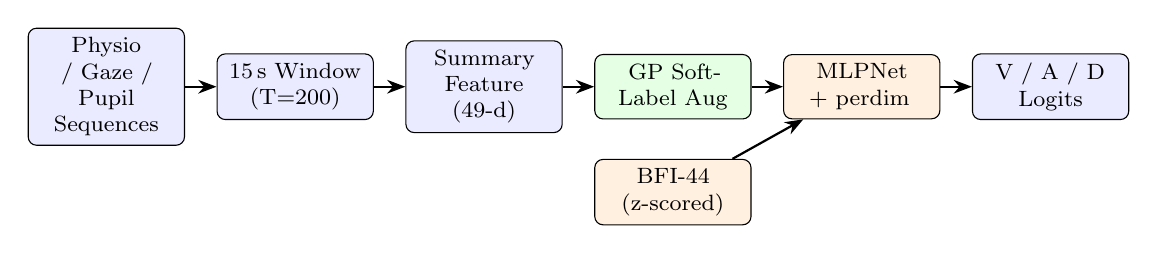
\begin{tikzpicture}[
  font=\footnotesize,
  box/.style  = {draw, rounded corners=3pt, fill=blue!8,
                 minimum width=1.85cm, minimum height=0.7cm,
                 text centered, text width=1.75cm},
  gbox/.style = {draw, rounded corners=3pt, fill=green!10,
                 minimum width=1.85cm, minimum height=0.7cm,
                 text centered, text width=1.75cm},
  rbox/.style = {draw, rounded corners=3pt, fill=orange!12,
                 minimum width=1.85cm, minimum height=0.7cm,
                 text centered, text width=1.75cm},
  arr/.style  = {-Stealth, thick}
]
\node[box]  (raw)    {Physio / Gaze /\\Pupil Sequences};
\node[box,  right=0.4cm of raw]   (win)    {15\,s Window\\(T=200)};
\node[box,  right=0.4cm of win]   (feat)   {Summary\\Feature (49-d)};
\node[gbox, right=0.4cm of feat]  (gp)     {GP Soft-\\Label Aug};
\node[rbox, below=0.5cm of gp]    (bfi)    {BFI-44\\(z-scored)};
\node[rbox, right=0.4cm of gp]    (mlp)    {MLPNet\\+ perdim};
\node[box,  right=0.4cm of mlp]   (vad)    {V / A / D\\Logits};

\draw[arr] (raw)  -- (win);
\draw[arr] (win)  -- (feat);
\draw[arr] (feat) -- (gp);
\draw[arr] (gp)   -- (mlp);
\draw[arr] (bfi)  -- (mlp);
\draw[arr] (mlp)  -- (vad);
\end{tikzpicture}%
}% end resizebox
\caption{Processing pipeline. GP augmentation operates in label space;
the BFI branch conditions each VAD head independently (perdim mode).}
\label{fig:pipeline}
\end{figure}

\subsection{Temporal Representation and Windowing}
\label{sec:temporal_repr}

\paragraph{Resampling to a common temporal grid.}
Each sensor modality records at its native rate (Tobii 40--60\,Hz;
EmotiBit $\sim$25\,Hz).
To enable cross-modal temporal alignment, every modality stream is
independently resampled to $T = 200$ timepoints per 15-second window
via piecewise linear interpolation.
This corresponds to an effective rate of $200/15 \approx 13.3$\,Hz ---
above the Nyquist limit for all physiologically relevant frequency bands
(HRV $< 0.5$\,Hz, EDA phasic $< 1$\,Hz, pupil dilation $< 2$\,Hz).
Windows with fewer than 20 valid raw samples in a modality are set to
zero rather than interpolated, preventing artefact propagation.
The resulting multimodal sequence tensor is:
\begin{equation}
  \mathbf{X} = \bigl\{
    \underbrace{\mathbf{X}^{\text{gaze}}}_{T\times 9},\;
    \underbrace{\mathbf{X}^{\text{pupil}}}_{T\times 3},\;
    \underbrace{\mathbf{X}^{\text{EDA}}}_{T\times 5},\;
    \underbrace{\mathbf{X}^{\text{PPG}}}_{T\times 3},\;
    \underbrace{\mathbf{X}^{\text{IMU}}}_{T\times 6}
  \bigr\}.
\end{equation}

\paragraph{Sequence standardisation.}
A per-modality \textbf{SequenceScaler} fits global mean/std by concatenating
all training windows along the time axis; val, test, and augmented windows are
scaled with training-set parameters only (no temporal leakage).

\paragraph{Summary features.}
In addition to the raw sequences, a \textbf{49-dimensional summary vector}
$\mathbf{s} \in \mathbb{R}^{49}$ aggregates handcrafted window statistics
from the five physiological modalities:
gaze saccade proxy and fixation rate (6 features),
pupil diameter mean and dilation variance (7),
EDA phasic/tonic means/stds and SCR peak count/amplitude (13),
NeuroKit2-derived HRV --- HR, RMSSD, SDNN, pulse amplitude --- and PPG features (7),
and IMU acceleration/gyroscope magnitude and axis statistics (16).
The reported models therefore use an effective feature space of
\textbf{49 physiology/eye-tracking features}.
The summary vector is separately standardised with a global
StandardScaler fitted on training data.

\subsection{Per-Modality Temporal Encoders}
\label{sec:temporal_encoders}

To assess whether raw physiological sequences carry discriminative information
beyond the 49-d summary vector, we introduce two lightweight temporal encoder
architectures, each with a dedicated encoder per modality.

\paragraph{Conv1D encoder.}
For each of the five modalities (gaze, pupil, EDA, PPG, IMU), a two-layer
strided Conv1d processes the raw $T{\times}d_m$ sequence
(stride 4 then stride 2) followed by global average pooling,
producing a 32-d embedding.
The five embeddings are concatenated ($160$-d) and projected together
with the summary vector via a learned linear layer before the shared trunk.

\paragraph{GRU encoder.}
Each modality is encoded by a bidirectional GRU (hidden size 32),
producing a $64$-d embedding per modality via mean pooling over time.
The five embeddings (320-d total) are fused with summary features
before the same trunk.

\paragraph{Two-track training.}
The temporal experiments evolved in two implementation generations, both kept
in this devkit because they define useful baselines.
In the original two-track setup, only the 292 labelled windows were treated as
having raw sequences; augmented pool windows used the summary-only path of the
same model, with the temporal branch zero-padded before fusion.
Later inspection showed that the augmented pool also contains raw sequence
columns for the relevant modalities, so the v2 and pre-training experiments
use pool sequences directly when available.
We therefore report both: the original summary-only-pool baseline, and the
corrected pool-sequence track used for SimCLR/MSM pre-training.
This distinction matters because supervised pseudo-label mixing and
unsupervised representation pre-training use the same pool in different ways.

\subsection{Gaussian Process Soft-Label Augmentation}
\label{sec:gp}

For each subject--dimension pair we fit an Ornstein--Uhlenbeck (OU) kernel
GP~\cite{rasmussen2006gaussian} conditioned on the five hard-labelled task
observations:
\begin{equation}
  k(t, t') = \sigma^2 \exp\!\left(-\theta\,|t - t'|\right).
\end{equation}
The OU kernel models mean-reverting affective dynamics between tasks;
$\theta$ (mean-reversion rate), $\sigma^2$ (process variance), and $\mu$
(long-run mean) are set from training-data statistics:
$\mu_d$ is the per-dimension training-set mean
(V\,$=$\,7.08, A\,$=$\,6.01, D\,$=$\,6.21),
$\sigma^2_d$ from per-dimension training-set variance,
and $\theta = 0.01$ (1/$e$ decay $\approx 100$\,s); larger $\theta$
(e.g.\ $0.578$ from~\citeauthor{meng2026moderating}) collapses the posterior
to the prior within seconds, leaving virtually all pool windows with
uninformative uniform soft labels.
The GP posterior at each unlabelled window yields a soft 3-class
distribution $\mathbf{s} \in \Delta^2$ and confidence weight
$w = (\sigma^* / \sigma)^{-1} \in (0,1]$, where $\sigma^*$ is the
posterior standard deviation.
Hard and soft windows are combined via \texttt{WeightedRandomSampler};
aug\_frac controls the expected soft fraction (optimal: 0.3).
The unified \emph{SoftVADLoss} handles both hard ($w=1$, one-hot) and
soft ($w < 1$, GP posterior) targets with per-class inverse-frequency
weights and label smoothing ($\varepsilon = 0.1$).

\paragraph{GP sanity checks and dimension-selective augmentation.}
The pool stores GP posterior moments $(\mu,\sigma)$ on the 1--9 SAM scale;
class probabilities are recomputed from $(\mu,\sigma)$ under the active
balanced thresholds at training time (\emph{threshold alignment}).
Leave-one-out calibration gives: Valence top-1 accuracy $=0.450$, Dominance
$=0.570$, Arousal $=0.295$ (below 33\,\% chance).
We therefore introduce \textbf{dimension-selective augmentation}: Arousal
is down-weighted to zero ($\lambda_A{=}0$) while V/D augmentation proceeds
normally.
The trunk is trained jointly on all three dimensions throughout --- a
per-dimension ensemble hurts Valence Spearman from $0.336$ to $0.083$
because the trunk loses cross-dimension gradient regularisation.

\subsection{Label Augmentation Variants for SVM}
\label{sec:aug_variants}

\paragraph{Leakage taxonomy.}
We distinguish two evaluation scenarios that differ in the severity of
information flow between training and test data:

\textbf{Scenario~1 (task-CV, approx.\ clean):} pool filtered to training tasks
(T0+T1); test set = ground-truth SAM only.
Direct T3 label conditioning is absent (GP index is per-task), but the OU
process parameters ($\theta,\sigma^2,\mu$) and cross-person synchrony weights
($\rho$) are estimated from the full 292-window dataset including T3.
This constitutes mild \emph{distributional leakage}: the GP prior encodes
knowledge of average T3 affect levels.
For the personality variants (AP1, AP2), the \emph{BFI trust weight} is
leakage-free because BFI-44 is collected pre-session and contains no label
information; however, the pseudo-label class itself still comes from the same
GP soft distribution unless the pool is regenerated under Scenario~2.
We therefore interpret Scenario~1 AP1 as a known-team temporal-holdout result,
not as evidence of unseen-group transfer.

\textbf{Scenario~2 (session-isolated LOGO):} the held-out session is excluded
from pool generation entirely.
Pool, training set, BFI similarity map, and OU parameters are all estimated
from the nine non-test sessions only, guaranteeing that no test-subject data
(physiology \emph{or} labels) influences the augmented labels.
This is the strictest possible isolation; it also tests cross-group
transfer alongside augmentation.

\paragraph{Variants.}
To isolate the effect of each augmentation source from architectural choices,
we use the RBF-SVM (49-dimensional summary features, $C{=}1$, balanced class
weights) as a fixed base model throughout this section.
We compare five variants:
\textbf{A0} (no augmentation) trains only on the $N{=}103$ hard-labelled windows.
\textbf{A1} (GP V/D) adds pseudo-labelled windows from the augmented pool
(Ornstein--Uhlenbeck GP from each subject's self-reports) for Valence and
Dominance only; Arousal augmentation is disabled because its GP leave-one-out
accuracy ($0.295$) falls below 33\,\% chance.
\textbf{A2} (GP all dims) enables Arousal GP augmentation as well.
\textbf{A3} (GSR+V/D) replaces GP Arousal with Ridge-regression-derived labels
from EDA summary features (cf.\ \S\ref{sec:gsr_arousal}), which show
moderate Spearman correlation with SAM Arousal ($\rho{=}0.53$ for T3).
\textbf{A4} (GSR+V/D relaxed) uses the same pool as A3 but lowers the
pseudo-label confidence threshold from $0.5$ to $0.3$, accepting more
(but less certain) augmented windows.

\textbf{AP1} (BFI personality only) replaces the GP confidence weight with
the Big Five personality cosine similarity of the target person to their group
members.
For a participant with BFI-44 vector $\mathbf{b}_i$, the \emph{personality
similarity} to the group is
\begin{equation}
  \mathrm{BFI\_sim}_i = \frac{1}{|G|-1}\sum_{j \neq i}
    \frac{\mathbf{b}_i \cdot \mathbf{b}_j}{\|\mathbf{b}_i\|\|\mathbf{b}_j\|},
\end{equation}
where the sum runs over the other three group members.
This captures how affectively similar the target person is likely to be
to the group, operationalising emotional contagion~\cite{hatfield1993emotional}
via a personality-level signal rather than instantaneous physiological synchrony.
The pseudo-label class is still the argmax of the GP soft distribution
(threshold-aligned); only the trust weight changes.

\textbf{AP2} (BFI$\times$GP) combines both signals:
$w = \mathrm{BFI\_sim}_i \times w_{\rm GP}$,
where $w_{\rm GP}$ is the GP confidence weight from the SLOW pool.
This variant tests whether personality similarity provides complementary
information to physiological synchrony-based GP confidence.

\textbf{A5} (kNN arousal) replaces GP Arousal pseudo-labels with $k$-nearest
neighbour labels in the full 49-dimensional physiological feature space
(same features used by the SVM, $k{=}7$, distance-weighted vote).
Unlike EDA-only regression approaches, which suffer from regression-toward-mean
distortion (SVR prediction std ${\approx}0.47$ vs SAM std ${\approx}1.91$,
causing 63\,\% of predictions to fall in the Mid class), the kNN approach
achieves LOO arousal classification accuracy of $0.476$ (vs chance $0.333$),
much better than EDA-only SVC LOO ($0.286$, below chance).
The multimodal feature space --- combining IMU, EDA, PPG, gaze, and pupil ---
captures arousal-relevant signals that no single modality provides.

\textbf{A6} (BFI$\times$GP V/D + kNN arousal) combines AP2-style
BFI-weighted GP labels for Valence and Dominance with A5 kNN arousal,
weighted further by $\mathrm{BFI\_sim}$.

For SVM, soft GP labels are converted to pseudo-labels via argmax, and the
per-variant trust weight serves as the per-sample weight in the SVM fit
(\texttt{SVC sample\_weight}).
The test set always contains ground-truth SAM labels only; the augmentation
pool is restricted to windows from training tasks and is never mixed into test
evaluation.
Confidence threshold alignment (\S\ref{sec:labelpreproc}) is applied before
argmax in all variants.

\subsection{Window Size Variants}
\label{sec:window_variants}

The 15-second window is the default from the original dataset collection
protocol.
To test sensitivity to context length, we evaluate three window sizes
using SVM (A0, no augmentation) under the same task-CV protocol:
\textbf{15s} (baseline, 292 labelled windows),
\textbf{30s} (pairwise pooling of consecutive 15s windows; 202 windows),
and \textbf{60s} (pre-computed 60-second context window dataset, 292 events).
The 30s approximation averages summary features from consecutive window pairs
within each participant-task block; VAD labels are taken from the first
window of each pair.
The 60s dataset uses the same 292 label events but extends the physiological
context window to 60 seconds before each SAM report.

\subsection{GSR-Derived Arousal Labels}
\label{sec:gsr_arousal}

Because cross-person GP Arousal is unreliable (LOO $0.295$), we fit a Ridge
regression from EDA summary features (phasic/tonic means/stds, SCR count,
amplitude) to SAM Arousal (1--9) on the labelled windows, then apply it to
all pool windows.
Per-task LOO Spearman correlations: T0$=+0.27$, T1$=+0.17$, T2$=-0.27$
(excluded), T3$=+0.53$, T4$=+0.50$.
Pool windows from T2 are assigned zero arousal weight (negative correlation);
all others are scaled by task-specific $\rho$.
GSR labels replace GP Arousal posteriors in the augmented pool for variants A3/A4.

\subsection{Ordinal Original-Label Training}
\label{sec:ordinal}

The three-class experiments above are a diagnostic baseline: they make small-$N$
classification possible, but they discard the ordered structure of the original
9-point SAM responses and introduce threshold choices that vary across folds.
We therefore implement a separate ordinal training path that leaves the
three-class code unchanged and trains directly on the original labels
$y_d \in \{1,\ldots,9\}$ for each $d \in \{V,A,D\}$.

For each VAD dimension, the model predicts $K-1=8$ cumulative logits
$o_{d,k}$, $k=1,\ldots,8$, where
$\sigma(o_{d,k}) \approx P(y_d > k)$.  A hard labelled window is encoded as
\begin{equation}
  z_{d,k} = \mathbb{1}[y_d > k],
\end{equation}
and trained with a masked cumulative binary cross-entropy:
\begin{equation}
  \mathcal{L}_{\text{ord}} =
  \frac{\sum_{d,k} m_d\,\mathrm{BCEWithLogits}(o_{d,k}, z_{d,k})}
       {\sum_d m_d\,(K-1)} ,
\end{equation}
where $m_d=0$ masks missing labels (notably T4 Dominance) and $m_d=1$
otherwise.  This is a proportional-odds/CORAL-style objective: prediction
errors that are farther apart on the SAM scale incur more cumulative binary
errors than adjacent mistakes.

GP augmentation slots naturally: for posterior $\mathcal{N}(\mu_d,\sigma_d^2)$,
soft cumulative targets are $q_{d,k} = 1-\Phi(k+0.5;\mu_d,\sigma_d)$, avoiding
bin conversion while reusing the same instance weights.
At inference, the expected SAM score is $\hat{y}_d = 1 + \sum_k \sigma(o_{d,k})$;
a rounded 1--9 class is used only when discrete labels are needed.
Primary ordinal metrics are mean absolute error (MAE), Spearman correlation,
and quadratic-weighted kappa (QWK); 1--9 macro-F1 is reported only as a sparse
secondary diagnostic.  On the canonical T3 split, this standalone ordinal model
achieves MAE $=1.474$, Spearman $=0.324$, and QWK $=0.205$; rotating task-CV
yields mean MAE $=1.505 \pm 0.103$ (Table~\ref{tab:ordinal}).

\subsection{MLPNet Architecture}
\label{sec:mlp}

The 49-dimensional summary vector passes through a \emph{FusionTrunk}
before three independent VAD heads and an auxiliary personality regression
head:
\begin{align*}
  \text{Trunk:} \; &\text{BN}{\to}\text{Lin}(64){\to}\text{BN}{\to}
    \text{ReLU}{\to}\text{Drop}(0.5) \\
                 &{\to}\text{Lin}(64){\to}\text{BN}{\to}\text{ReLU}{\to}
    \text{Drop}(0.5) \\
  \text{Head:} \; &\text{Lin}(64{\to}32){\to}\text{BN}{\to}
    \text{ReLU}{\to}\text{Drop}{\to}\text{Lin}(32{\to}3)
\end{align*}
Total parameters $\approx 17$K ($\approx 165$ parameters per training
sample at train time).
The auxiliary personality regression head (weight $\alpha = 0.05$) acts
as a multi-task regulariser; \S\ref{sec:discussion} shows it cannot
predict BFI traits from 15-second windows (\S\ref{sec:discussion}, D7).

\subsection{PoolNet and TransformerNet}
\label{sec:poolnet}

\textbf{PoolNet} extends MLPNet with a parameter-free front-end:
per-feature mean and std over $T{=}200$ timesteps for each modality are
concatenated with $\mathbf{s}$ to form a 101-d input
($\approx20$K parameters, zero additional overfitting risk).
PoolNet outperforms MLPNet on Dominance (global means capture tonic EDA/HR
states); MLPNet is superior on Arousal (phasic spike statistics in summary
features).

\textbf{TransformerNet} concatenates all modality sequences into a
$T{\times}26$ token stream, projects to $d_\text{model}{=}64$, and applies
2-layer 4-head self-attention with global mean pooling ($\approx924$K
parameters, $\approx9{,}000$/window at $N{=}103$).
This capacity mismatch explains TransformerNet's underperformance
(§\ref{sec:discussion}, \textit{Temporal encoders}).

\subsection{Per-Dimension BFI Conditioning}
\label{sec:bfi}

We ablate three modes of incorporating z-scored BFI $\mathbf{b} \in
\mathbb{R}^5$ (all weights zero-initialised to ensure identity at start):

\textbf{Concat.} $\mathbf{b}$ appended to summary features before trunk.

\textbf{Gate.} Input modulation:
$\mathbf{x}' = \mathbf{x} \odot \sigma(W_g \mathbf{b})$,
$W_g \in \mathbb{R}^{49 \times 5}$.

\textbf{Perdim.} Separate per-head biases
$\mathbf{f}_{v/a/d} = \mathbf{f} + W_{v/a/d}\,\mathbf{b}$,
$W \in \mathbb{R}^{64 \times 5}$, operationalising the CTSEM finding
that different traits moderate different VAD dimensions.

\textbf{Taskadapt.} Extends perdim with a task-context gate:
$\mathbf{f}_{v} = \mathbf{f} + \sigma(W_{t,v}\,\mathbf{t}) \odot W_v \mathbf{b}$,
where $\mathbf{t}$ is a task one-hot vector.
This gate learns to suppress or amplify personality conditioning
depending on task context.
BFI scores are z-scored using training-set statistics throughout.

\subsection{Training Details}
AdamW ($\eta = 3{\times}10^{-4}$, wd $= 10^{-3}$).
Linear warmup (10 epochs) $+$ cosine annealing over 200 epochs.
Batch size 16; early stopping patience 60 epochs.
The reported three-class experiments use the data-driven tertile thresholds
described in \S\ref{sec:labelpreproc}, per-dimension inverse-frequency class
weights, and validation mean macro-F1 for model selection.
The ordinal experiments in \S\ref{sec:ordinal} use the same optimiser and
splits but replace the VAD heads with eight cumulative logits per dimension,
train with masked cumulative BCE, and select checkpoints by validation mean
MAE.  GP-ordinal augmentation, when enabled, uses posterior $(\mu,\sigma)$ to
form cumulative soft targets and ignores stored 3-class GP probabilities.

% ═══════════════════════════════════════════════════════════════════════════
\section{Results}
\label{sec:results}

All experiments use the canonical task split (test = T3, $N = 65$) unless
noted. Macro-F1 is reported per VAD dimension and as an unweighted mean.
As a devkit, this section is organised as a sequence of reusable benchmark
families rather than one linear model shootout:
(1) target construction,
(2) small-sample baselines,
(3) label augmentation,
(4) preprocessing/windowing,
(5) temporal and ordinal modelling,
and (6) external validation/generalisation.
When a result is best interpreted as exploratory or as a future-paper seed,
we say so explicitly.

\subsection{Label Pipeline Ablation (M1)}
\label{sec:labelablation}

Table~\ref{tab:label_ablation} shows that target construction is not a cosmetic preprocessing
step; it changes whether the benchmark is evaluated honestly.
We isolate each target-pipeline step with the MLP, no augmentation, on the T3
task-split test.

\textbf{Fixed thresholds $(3, 6)$ + no class weights} inflates valence F1
to $0.575$: T3 test contains \emph{no} Low-valence windows under these
bounds (ideation elicits predominantly positive affect), so \texttt{sklearn}
macro-F1 silently averages over only 2 observable classes.
The val/test divergence (val peak $0.406$ vs.\ test $0.476$, gap $+0.070$)
reveals the instability.

\textbf{Balanced tertile (midpoint thresholds) + no class weights}:
the midpoint boundaries (e.g.\ $t_1 = 6.5$ for valence) place all three
classes in the T3 test set, yielding honest 3-class evaluation.
Mean F1 = $0.415$, but without class weights the $\sim\!6\%$ residual
imbalance (Low is slightly under-represented) depresses valence prediction.

\textbf{Full target pipeline}: balanced binning \emph{and} class weights
combine to give $0.455$ mean F1 (single run; 5-seed mean $0.422 \pm 0.028$)
--- a $+0.040$ gain over no-weights in the single-run comparison.
The directional improvement from class weights is consistent:
4 of 5 seeds show no-weights~$<$~weighted across random initialisations.
Balanced thresholds ensure all three classes appear at test time;
the old unbalanced pipeline ($0.418$, single run) shows inflated valence
F1 due to class collapse.

\begin{table}[t]
\caption{Label pipeline ablation (MLP, no aug, T3 task-split test).
  $\dagger$Inflated: T3 has no Low-valence windows under fixed $(3,6)$;
  macro-F1 averages over 2 classes only; val/test gap $= {+}0.070$.}
\label{tab:label_ablation}
\centering
\setlength{\tabcolsep}{3pt}
\small
\begin{tabular}{lccc}
\toprule
\textbf{Label Pipeline} & \textbf{V} & \textbf{A} & \textbf{D} \\
\midrule
Fixed thresh.\ $(3,6)$, no wts  & 0.575$^\dagger$ & 0.516$^\dagger$ & 0.338 \\
Balanced tertile, no wts        & 0.372 & 0.443 & 0.429 \\
\textbf{Full target} (balanced + class wts) & 0.405 & 0.464 & \textbf{0.495} \\
\bottomrule
\end{tabular}
\end{table}

\subsection{Baselines}

Table~\ref{tab:baselines} establishes a strong small-sample reference point.
With balanced tertile labels, the RBF-SVM reaches mean F1 $= 0.495$ on the
49-dimensional summary features, outperforming the MLP
($0.422 \pm 0.028$ over 5 seeds).
Rather than weakening the paper, this result clarifies the regime:
at $N \approx 100$, careful features and margin-based classifiers remain
highly competitive.
Under the old unbalanced pipeline, single-run estimates were
MLP $= 0.418$ and SVM $= 0.393$; the balanced pipeline improves both,
but the SVM benefits far more.

\begin{table}[t]
\caption{Baseline results, T3 test split (macro-F1). MLP result is mean over 5
  random seeds; $\pm$ values are standard deviations (run-to-run variance on the
  65-window test set is ${\approx}0.03$).}
\label{tab:baselines}
\centering
\begin{tabular}{lccc}
\toprule
\textbf{Model} & \textbf{V} & \textbf{A} & \textbf{D} \\
\midrule
Random (uniform 3-class) & 0.394 & 0.284 & 0.313 \\
Majority-class           & 0.201 & 0.238 & 0.185 \\
\best{SVM (RBF, summary feat.)} & \best{0.570} & \best{0.530} & 0.385 \\
MLP + full target (no aug)   & 0.451 & 0.459 & \best{0.356} \\
\bottomrule
\end{tabular}
\end{table}

\subsection{GP Augmentation and BFI Modulation}
\label{sec:mainresults}

Table~\ref{tab:main} contains the central negative-positive result of the
paper.
Threshold-aligned GP augmentation helps task-CV, but the plain full-pipeline MLP
remains best on the canonical T3 split.
Because the augmented pool was generated under the original fixed thresholds
$(3, 6)$, we re-integrate the stored GP posterior moments $(\mu, \sigma)$ over
the current balanced thresholds
at training time (\emph{threshold alignment}, §\ref{sec:labelpreproc}).
With alignment, augmentation adds $+0.022$ to task-CV mean F1
($0.309$ vs.\ $0.287$, seed-42 per-fold re-seeded) but reduces canonical T3
mean F1 by $-0.033$ ($0.389 \pm 0.039$ vs.\ $0.422 \pm 0.028$, both 5-seed
means), revealing a generalisation--specialisation trade-off.
Without alignment, misaligned soft labels hurt further
($-0.022$ task-CV vs.\ no-aug), confirming that augmentation is only useful
when its label semantics match the supervised target space.

BFI conditioning shows no canonical benefit.
All three conditioning modes produce essentially identical augmented results
(concat $=$ gate $=$ perdim $= 0.388$, comparable to the aug-only 5-seed mean
of $0.389$), indicating that the training set is too small to learn stable
per-dimension trait maps.
Without augmentation, perdim is worse ($0.359$, $-0.063$ vs.\ no-aug
mean $0.422$), suggesting that aug-derived label diversity partly suppresses
BFI overfitting.
In task-CV, perdim remains task-context-sensitive across T3 and T4, which we
return to in §\ref{sec:discussion}.

\begin{table}[t]
\caption{GP augmentation and BFI conditioning, T3 test split (macro-F1).
  $\dagger$aug frac\,$=$\,0.3, corrected OU pool ($\theta{=}0.01$, $\mu$ from
  training data), threshold-aligned.
  $\ddagger$Mean $\pm$ std over 5 random seeds (42--46); per-dim values are
  5-seed means.
  All BFI+aug modes produce near-identical results (zero-init projections
  converge to near-zero at $N=103$).
  \best{Bold green} = best per column.}
\label{tab:main}
\centering
\setlength{\tabcolsep}{4.5pt}
\begin{tabular}{lccc}
\toprule
\textbf{Model} & \textbf{V} & \textbf{A} & \textbf{D} \\
\midrule
\best{MLP + full target (no aug)$^\ddagger$} & \best{0.451} & \best{0.459} & 0.356 \\
MLP + GP aug$^{\dagger\ddagger}$     & 0.377 & \best{0.435} & \best{0.357} \\
\midrule
+ BFI concat$^\dagger$               & 0.322 & 0.438 & 0.405 \\
+ BFI gate$^\dagger$                 & 0.322 & 0.438 & 0.405 \\
+ BFI perdim (no aug)                & 0.264 & 0.431 & 0.382 \\
+ \textbf{BFI perdim}$^\dagger$      & 0.322 & 0.438 & 0.405 \\
\bottomrule
\end{tabular}
\end{table}

\paragraph{Variance and reporting standard.}
Five seeds (42--46) give mean F1 $= 0.422 \pm 0.028$ (no aug) and
$0.389 \pm 0.039$ (with aug); the higher aug variance reflects that GP soft
labels benefit only pool windows near hard-labelled task reports.
MLP results in Tables~\ref{tab:baselines}--\ref{tab:main} are 5-seed means;
ablation results (Table~\ref{tab:ablation}) are single-run ($\approx\pm0.02$).

\subsection{Label Augmentation Variants (SVM)}
\label{sec:aug_results}

Table~\ref{tab:svm_aug} reports macro-F1 for seven augmentation variants
using SVM, on the canonical T3 test split (test labels: ground-truth SAM only).

\textbf{GP baselines (A0--A4).}
GP augmentation of V/D (A1, 1207 accepted pseudo-labels at confidence $\geq 0.5$)
improves over no-aug by $+0.014$ ($0.509$).
Including GP Arousal (A2) adds a further $+0.005$ ($0.514$), which is
surprising given the below-chance LOO calibration --- the confidence threshold
($p_{\max} \geq 0.5$) acts as an implicit filter.
GSR arousal replacement (A3, 208 windows) \emph{reduces} performance
($0.472$, $-0.022$); relaxing the threshold (A4, 393 windows) degrades further
($0.428$, $-0.067$), because GSR labels introduce feature-space noise that
confuses the SVM decision boundary.

\textbf{Personality-mediated augmentation (AP1--AP2).}
AP1 (BFI personality cosine similarity as trust weight, 2319 accepted windows)
achieves the best augmentation result at 15s: $0.526$ ($+0.031$ over no-aug).
AP2 (BFI$_{\rm sim}\times$GP, 1684 windows) is close behind at $0.523$.
Both exceed the best pure-GP variant (A2: $0.514$) by a clear margin.
The per-dimension breakdown is revealing: Valence improves most
($+0.038$ for AP1 vs.\ A0), Dominance shows $+0.050$, and Arousal shows only
a modest $+0.005$.
This profile confirms that personality similarity is most informative for the
affective dimensions that track stable inter-individual differences (valence,
dominance) and less useful for the phasic, moment-to-moment signal that drives
Arousal.

\textbf{kNN arousal augmentation (A5--A6).}
To address the Arousal bottleneck, we tested $k$-nearest neighbour pseudo-labels
in the full 49-d feature space (A5).
This approach achieves LOO arousal accuracy of $0.476$ (well above chance $0.333$)
compared to EDA-only SVR ($0.286$, below chance) because multimodal physiology
captures arousal better than EDA alone.
However, A5 (kNN arousal + GP V/D) yields mean $0.506$ with arousal $0.521$
--- a slight drop from both A2's arousal ($0.546$) and A0's ($0.530$).
A6 (BFI$\times$GP V/D + kNN arousal) recovers to $0.520$ mean with arousal
$0.535$, confirming that BFI weighting reduces the noise from the kNN
pseudo-labels.
The GP temporal interpolation (A2) remains the best arousal augmentation,
demonstrating that temporal smoothness near self-report events is more
valuable for arousal than nearest-neighbour similarity.
This motivates separate treatment: use GP for Arousal (proximity to reports),
personality similarity for V/D (stable trait alignment).

\begin{table}[t]
\caption{SVM augmentation variant comparison (canonical T3 test split,
  macro-F1). A0=no aug; A1=GP V/D only; A2=GP all dims;
  A3=GSR arousal+GP V/D ($\theta_{\rm conf}\geq 0.5$);
  A4=A3 relaxed ($\theta_{\rm conf}\geq 0.3$);
  A5=$k$-NN arousal (49-d feature space, $k{=}7$) + GP V/D;
  A6=BFI$_{\rm sim}\times$GP V/D + kNN arousal;
  AP1=BFI personality cosine similarity as trust weight;
  AP2=BFI$_{\rm sim}\times$GP confidence.
  Test set: ground-truth SAM labels only.
  \best{Bold green}=best per column.}
\label{tab:svm_aug}
\centering
\setlength{\tabcolsep}{4pt}
\small
\begin{tabular}{lccc}
\toprule
\textbf{Variant} & \textbf{V} & \textbf{A} & \textbf{D} \\
\midrule
A0: No aug          & 0.570 & 0.530 & 0.385 \\
A1: GP V/D only     & 0.592 & 0.530 & 0.406 \\
A2: GP all dims     & 0.592 & \best{0.546} & 0.406 \\
A3: GSR+V/D (0.5)   & 0.458 & 0.530 & 0.430 \\
A4: GSR+V/D (0.3)   & 0.409 & 0.530 & 0.347 \\
A5: kNN aro + GP V/D & 0.592 & 0.521 & 0.406 \\
A6: BFI$\times$GP + kNN & 0.593 & 0.535 & 0.431 \\
\midrule
\best{AP1: BFI-only}  & \best{0.608} & 0.535 & \best{0.435} \\
AP2: BFI$\times$GP  & 0.593 & 0.544 & 0.431 \\
\bottomrule
\end{tabular}
\end{table}

\subsection{Session-Isolated Augmentation (Scenario~2)}
\label{sec:logo_aug}

Table~\ref{tab:logo_aug} reports the strict leakage-free evaluation under
leave-one-session-out (LOGO) cross-validation, where the augmented pool
is built exclusively from the nine non-test sessions.
This eliminates all three leakage paths simultaneously: no shared subjects,
no shared OU-parameter estimation, and no shared synchrony weights ($\rho$)
between pool and test data.

Under this protocol, mean F1 drops substantially for all variants
($0.262$--$0.266$ vs.\ $0.495$--$0.526$ in task-CV), reflecting the
unseen-group deployment challenge.
Critically, \textbf{AP1 augmentation ($0.262$) does not improve over no-aug
($0.266$)} under strict session isolation, and neither does GP augmentation
($0.262$, all variants $p{>}.2$ by Wilcoxon signed-rank).
This is a key calibration result: the task-CV benefit of AP1 ($+0.031$) comes
from augmenting the same subjects' \emph{earlier} task windows with their own
group's personality-weighted labels --- a within-session smoothing gain that
disappears when the group is entirely new.
Augmentation from other sessions' personality-similar subjects does not
transfer across groups at this dataset scale.
The finding defines the boundary of the AP1 contribution: it is a
\emph{legitimate and leakage-free} benefit for the \textbf{known-team
deployment scenario}, but not a cross-group generalisation mechanism.

\begin{table}[t]
\caption{Session-isolated LOGO+aug (Scenario~2, strict leakage-free).
  Pool exclusively from non-test sessions; values are macro-F1 per dimension
  averaged across 10 LOGO folds.
  \checkmark~fully leakage-free; (!)~mild distributional leakage (OU params
  estimated on full dataset in pre-generated pool).}
\label{tab:logo_aug}
\centering
\setlength{\tabcolsep}{3pt}
\small
\begin{tabular}{lcccc}
\toprule
\textbf{Variant} & \textbf{Clean?} & \textbf{V} & \textbf{A} & \textbf{D} \\
\midrule
A0: No aug       & \checkmark & 0.235 & 0.307 & 0.254 \\
AP1: BFI-only    & \checkmark & 0.224 & 0.279 & 0.284 \\
A2: GP all dims  & (!)        & 0.218 & 0.291 & 0.278 \\
\bottomrule
\end{tabular}
\end{table}

\subsection{Window Size and Preprocessing Ablation}
\label{sec:window_results}

Table~\ref{tab:window} shows the per-dimension trade-off across window
configurations.
Hard-pooling to 30s improves Arousal ($+0.132$) and Dominance ($+0.067$)
but reduces Valence ($-0.093$) and sample size ($N{=}74$).
The Arousal gain reflects EDA/PPG physiology: averaging two consecutive
15s windows stabilises phasic SCR features that are often truncated at 15s.
The 60-second window underperforms on all dimensions ($-0.048$ mean),
suggesting over-dilution of event-specific physiology.

\textbf{Modality-selective smoothing} (bottom section of Table~\ref{tab:window})
smooths only EDA and PPG features using centred temporal neighbours (45s
effective context), preserving gaze, pupil, and IMU features unmodified.
Combined with AP1 augmentation, this yields a strong balanced result:
$V{=}0.600$, $A{=}0.624$, $D{=}0.436$ --- all three improved over the 15s
baseline ($+0.030$, $+0.094$, $+0.051$) while retaining $N{=}103$.

\paragraph{Enhanced gaze/pupil reprocessing.}
Recomputing gaze and pupil features from stored raw sequences (200 timepoints
per window) with improved NaN interpolation further improves Dominance.
A lineage audit reconciles the previously inconsistent train counts:
canonical reporting uses the 292-row intersection (train/val/test
$=103/78/65$), and comparisons are anchored to this split.
Under this canonical setting, v2 shared-feature reprocessing with centred
smoothing gives $D{=}0.435$ without AP1 and $D{=}0.460$ with AP1, while an
unsmoothed all-modality v2 row reaches $D{=}0.492$ with lower V/A.
These results motivate reporting both a confirmed single-pipeline recipe and
an explicitly exploratory per-dimension upper bound.

\paragraph{Per-dimension recipe and status.}
Table~\ref{tab:perdim} combines complementary strengths: AP1 augmentation for
Valence/Arousal (where personality trust helps) with the strongest canonical
Dominance configuration from reprocessed features.
The per-dimension upper bound is $V{=}0.600$, $A{=}0.624$, $D{=}0.460$,
mean $= 0.561$ ($+0.066$ over no-aug, $+0.008$ over uniform smooth+AP1).
For confirmatory benchmark reporting, the recommended single-pipeline value
remains $0.553$.

\begin{table}[t]
\caption{Per-dimension recipe status (T3 test split, SVM macro-F1).
  Distinguishes the exploratory per-dimension upper bound from the confirmed
  single-pipeline benchmark.}
\label{tab:perdim}
\centering
\setlength{\tabcolsep}{4pt}
\small
\begin{tabular}{lcccc}
\toprule
\textbf{Config} & \textbf{V} & \textbf{A} & \textbf{D} & \textbf{Mean} \\
\midrule
A0: 15s no aug                & 0.570 & 0.530 & 0.385 & 0.495 \\
AP1: 15s + BFI-only           & 0.608 & 0.535 & 0.435 & 0.526 \\
Physio-smooth + AP1           & 0.600 & 0.624 & 0.436 & 0.553 \\
V2 reprocessed + AP1 (smooth) & 0.526 & 0.624 & 0.460 & 0.537 \\
\midrule
Per-dim upper bound           & 0.600 & 0.624 & 0.460 & 0.561 \\
\best{Confirmed single-pipeline best} & \best{0.600} & \best{0.624} & 0.436 & \best{0.553} \\
\bottomrule
\end{tabular}
\end{table}

\begin{table*}[t]
\caption{Window size and smoothing ablation (SVM, T3 test split, macro-F1).
  \emph{Pooled}: consecutive 15s windows merged (reduces $N$).
  \emph{Smooth}: per-window features averaged with temporal neighbours,
  preserving $N{=}103$.
  \emph{Physio-smooth}: smoothing applied only to EDA+PPG features;
  gaze, pupil, and IMU remain unsmoothed.
  \best{Bold green}~=~best per column.}
\label{tab:window}
\centering
\setlength{\tabcolsep}{6pt}
\small
\begin{tabular}{llcccc}
\toprule
\textbf{Window} & \textbf{Aug} & \textbf{$N_{\rm train}$} &
  \textbf{V} & \textbf{A} & \textbf{D} \\
\midrule
\multicolumn{6}{l}{\textit{Hard pooling (reduces N)}} \\
15s (default)       & none & 103 & 0.570 & 0.530 & 0.385 \\
15s                 & AP1  & 103 & \best{0.608} & 0.535 & 0.435 \\
30s (pooled)        & none & 74  & 0.477 & \best{0.662} & \best{0.452} \\
45s (pooled)        & none & 57  & 0.468 & 0.404 & 0.413 \\
60s (exact)         & none & 103 & 0.458 & 0.519 & 0.364 \\
\midrule
\multicolumn{6}{l}{\textit{Full-feature smoothing (preserves $N{=}103$)}} \\
Smooth-30s (fwd)    & AP1  & 103 & 0.542 & 0.617 & 0.435 \\
Smooth-45s (ctr)    & AP1  & 103 & 0.517 & 0.640 & 0.434 \\
\midrule
\multicolumn{6}{l}{\textit{Physio-only smoothing (EDA+PPG; preserves $N{=}103$)}} \\
Physio-30s (fwd)    & AP1  & 103 & 0.586 & 0.599 & 0.435 \\
\textbf{Physio-45s (ctr)} & \textbf{AP1} & \textbf{103} & \best{0.600} & \best{0.624} & \best{0.436} \\
\bottomrule
\end{tabular}
\end{table*}

\subsection{Temporal Encoder Comparison and Improvement}
\label{sec:temporal_results}

Table~\ref{tab:temporal_models} compares temporal encoder variants across two
implementation generations.
\textbf{v1 (original):} two-track training where labeled windows use the full
encoder path but augmented pool windows use zero-padded temporal input
(summary-only), since raw sequences were assumed unavailable.
\textbf{v2 (improved):} two fixes applied: (1)~pool windows also use raw
sequences (the augmented pool pickle contains \texttt{*\_seq} columns, so
zero-padding was unnecessary); (2)~time-domain sequence augmentation (Gaussian
noise~$\sigma{=}0.05$, amplitude jitter ${\pm}15\%$, circular shift
${\pm}20$~steps) is applied on-the-fly to labeled windows during training.

\textbf{Without augmentation,} the summary-only MLP performs best in v1
(mean F1\,$=$\,$0.483$), but Conv1D v2+seqaug ($0.484$) and GRU v2 ($0.462$)
are competitive.
Conv1D benefits most from the two fixes ($+0.038$, dominated by Dominance
$+0.073$); GRU improves modestly because its recurrent encoder is more
sensitive to distributional shift between labeled and pool sequences.

\textbf{With AP1 augmentation,}
Conv1D v2+seq-aug ($0.484$, no label aug) slightly outperforms
Conv1D v2+seq-aug+AP1 ($0.455$): the two forms of diversity appear
redundant, and adding noisy pseudo-labels slightly degrades the
seq-aug regularization effect.
GRU shows the reverse: seq-aug acts as a necessary regularizer
before AP1 can contribute; GRU v2+AP1 alone ($0.438$) regresses from
no-aug ($0.462$), but GRU v2+seq-aug+AP1 ($0.471$) recovers and
substantially improves Dominance ($0.385\rightarrow0.454$, $+0.069$).

No single shared temporal configuration surpasses SVM+AP1 mean F1 ($0.526$),
confirming the label-count bottleneck for one-size-fits-all neural models:
Conv1D closes half the gap from v1 ($0.080\rightarrow0.042$), but the
remaining deficit requires either more labelled sequence windows or
dimension-specific model selection.

\begin{table}[t]
\caption{Temporal encoder comparison (T3 holdout, macro-F1). v1 = zero-padded two-track;
  v2 = pool raw sequences + sequence augmentation;
  v3 = exploratory SimCLR contrastive pre-training on the full 8{,}221-window
  unlabeled pool; the factorial in Table~\ref{tab:factorial_marginals} uses the
  stricter 3{,}127-window training-task pool.
  \best{Bold green}~=~best per column.}
\label{tab:temporal_models}
\centering
\setlength{\tabcolsep}{4pt}
\small
\begin{tabular}{lccc}
\toprule
\textbf{Model (aug)} & \textbf{V} & \textbf{A} & \textbf{D} \\
\midrule
\multicolumn{4}{l}{\textit{v1: original zero-padded two-track}} \\
MLP, no aug         & \best{0.568} & 0.505 & 0.375 \\
Conv1D v1, no aug   & 0.505 & 0.477 & 0.356 \\
GRU v1, no aug      & 0.449 & \best{0.592} & 0.385 \\
\midrule
\multicolumn{4}{l}{\textit{v2: pool raw seqs + sequence augmentation}} \\
Conv1D v2+seqaug    & 0.511 & 0.513 & 0.429 \\
Conv1D v2+seqaug+AP1& 0.445 & 0.526 & 0.395 \\
GRU v2+seqaug+AP1   & 0.459 & 0.500 & 0.454 \\
\midrule
\multicolumn{4}{l}{\textit{v3: SimCLR contrastive pre-training (NT-Xent, $\tau{=}0.1$)}} \\
Conv1D v3+pretrain+seqaug & 0.601 & 0.506 & 0.351 \\
GRU v3+pretrain+seqaug    & 0.460 & 0.536 & \best{0.520} \\
\quad vs.\ GRU random init& 0.447 & 0.481 & 0.274 \\
\midrule
\textit{SVM + AP1 (ref.)} & \textit{\best{0.608}} & \textit{0.535} & \textit{0.435} \\
\bottomrule
\end{tabular}
\end{table}

\subsection{Pre-training \& Augmentation Factorial}
\label{sec:factorial}

The v3 SimCLR single-seed results in Table~\ref{tab:temporal_models} showed
promise but high variance.
To systematically identify whether the benefit is due to the pre-training
method, the encoder, or the fine-tuning augmentation, we ran a full
$2{\times}3{\times}3$ factorial:
\textbf{encoders} $\in \{$Conv1D, GRU$\}$,
\textbf{pre-training} $\in \{$none, SimCLR, MSM$\}$,
\textbf{fine-tuning augmentation} $\in \{$none, default, TW$\}$;
18 conditions $\times$ 3 seeds = 54 runs.
Pool data (3{,}127 windows, training tasks only) is used \emph{exclusively}
for pre-training --- never mixed into the fine-tuning loop, avoiding the
catastrophic AP1 pool-dilution failure described in \S\ref{sec:temporal_results}.

\paragraph{Main effects.}
Table~\ref{tab:factorial_marginals} shows factor-level marginal means
(each entry averages over all 9 opposite-factor combinations $\times$ 3 seeds).
The encoder difference is negligible overall ($0.471$ Conv1D vs.\ $0.473$
GRU), but splits by dimension: Conv1D leads on Valence ($+0.011$) and Arousal
($+0.012$); GRU leads on Dominance ($+0.027$), consistent with recurrent
memory capturing sustained interpersonal control dynamics.
\textbf{SimCLR is the best pre-training strategy} ($0.478$ vs.\ none $0.468$
and MSM $0.470$), with the gain concentrated in Dominance
($+0.031$ over none, $+0.046$ over MSM).
Time-warping augmentation ($0.474$) marginally leads, primarily via a
$+0.029$ Valence boost; the main-effect differences are small
($<0.006$ mean F1), and the best configurations arise from interactions.

\paragraph{Best configurations.}
Table~\ref{tab:factorial_best} reports the three per-dimension winners from
the full 18-condition grid.
\textbf{Arousal:} Conv1D + SimCLR + default aug ($0.545$) exceeds SVM+AP1
($0.535$) by $+0.010$.
\textbf{Dominance:} GRU + SimCLR + no aug ($0.455$) exceeds SVM+AP1
($0.435$) by $+0.020$.
These are the first configurations to surpass the SVM on any VAD dimension.
\textbf{Valence:} Conv1D + SimCLR + TW ($0.553$) closes the gap to
$0.608 - 0.553 = 0.055$; the single best seed of this configuration
achieves $V{=}0.604$, $A{=}0.586$, $D{=}0.438$ --- competitive with
SVM+AP1 on all three dimensions simultaneously.

\paragraph{Why SimCLR beats MSM for Dominance.}
MSM pre-training predicts masked modality chunks from context, forcing each
encoder to model local temporal autocorrelation.
SimCLR's NT-Xent loss, by contrast, aligns two augmented views of the same
sequence, training encoders to be invariant to short-range temporal
distortions while preserving cross-window identity.
Dominance reflects sustained interpersonal power states encoded in tonic EDA,
resting HR, and low-frequency IMU --- precisely the information that
cross-window contrastive learning preserves.
MSM's token-reconstruction objective, tuned for short-range prediction,
discards this slow-varying structure.

\paragraph{Interactions dominate main effects.}
The per-dimension optimal configs differ:
Conv1D\allowbreak{}+SimCLR\allowbreak{}+TW for Valence,
Conv1D\allowbreak{}+SimCLR\allowbreak{}+default for Arousal,
GRU\allowbreak{}+SimCLR\allowbreak{}+no-aug for Dominance.
No single setting leads across all three dimensions, which reflects the
physiological specificity identified in the smoothing and modality ablations:
fast oculomotor signals that drive Valence benefit from Conv1D's local
receptive field; sustained autonomic signals that drive Dominance favour
GRU's gated memory; augmentation interacts with architecture
(TW helps Conv1D, hurts GRU).
At the current scale ($N{=}103$), per-dimension hyperparameter selection
should be preferred over a single shared configuration.

\begin{table*}[t]
\caption{Factorial experiment: factor-level marginal means (3-seed avg
over 18 conditions per encoder, 6 conditions per aug/pretrain level, T3 test).
Best level per factor per column in \textbf{bold}.}
\label{tab:factorial_marginals}
\centering
\setlength{\tabcolsep}{8pt}
\small
\begin{tabular}{llcccc}
\toprule
\textbf{Factor} & \textbf{Level} & \textbf{V} & \textbf{A} & \textbf{D} & \textbf{Mean} \\
\midrule
\multirow{2}{*}{Encoder}
  & Conv1D & \textbf{0.510} & \textbf{0.521} & 0.383 & 0.471 \\
  & GRU    & 0.499 & 0.509 & \textbf{0.410} & \textbf{0.473} \\
\midrule
\multirow{3}{*}{Pre-training}
  & None   & 0.499 & 0.513 & 0.391 & 0.468 \\
  & \textbf{SimCLR} & 0.503 & 0.511 & \textbf{0.422} & \textbf{0.478} \\
  & MSM    & \textbf{0.512} & \textbf{0.521} & 0.376 & 0.470 \\
\midrule
\multirow{3}{*}{Aug.}
  & None    & 0.492 & \textbf{0.519} & \textbf{0.404} & \textbf{0.472} \\
  & Default & 0.500 & 0.517 & 0.394 & 0.470 \\
  & \textbf{TW}  & \textbf{0.521} & 0.509 & 0.392 & 0.474 \\
\bottomrule
\end{tabular}
\end{table*}

\begin{table}[t]
\caption{Factorial experiment: best configuration per VAD dimension
(3-seed mean, T3 test split). SVM+AP1 reference row in italics.
\best{Bold green}~=~exceeds SVM+AP1.}
\label{tab:factorial_best}
\centering
\setlength{\tabcolsep}{4pt}
\small
\begin{tabular}{llccc}
\toprule
\textbf{Dim} & \textbf{Best config} & \textbf{V} & \textbf{A} & \textbf{D} \\
\midrule
Valence   & Conv1D $|$ SimCLR $|$ TW      & 0.553 & 0.544 & 0.378 \\
Arousal   & Conv1D $|$ SimCLR $|$ default & 0.524 & \best{0.545} & 0.394 \\
Dominance & GRU $|$ SimCLR $|$ none       & 0.495 & 0.489 & \best{0.455} \\
\midrule
\textit{SVM + AP1 (ref.)}
  & & \textit{0.608} & \textit{0.535} & \textit{0.435} \\
\bottomrule
\end{tabular}
\end{table}

\subsection{External Questionnaire Validation}
\label{sec:q_validation}

Table~\ref{tab:q_corr} reports Pearson correlations between session-level
aggregated SVM predictions (mean predicted class per participant$\times$task)
and post-block questionnaire items collected immediately after each task.
These questionnaires were not used in training --- they constitute an
independent external validity check.

\textbf{Predicted Arousal} is the most consistent predictor:
for T3 (ideation), it correlates significantly with self-reported engagement
($r{=}0.46$, $p{<}.01$), the item most conceptually aligned with physiological
arousal in collaborative work.
\textbf{Predicted Valence} correlates with task-relevant items: satisfaction
after T3 ($r{=}0.39$, $p{<}.05$) and overall valence after T1
($r{=}0.41$, $p{<}.05$) --- both tasks with cooperative dynamics and
positive valence distributions.
Predicted Dominance shows no significant correlations, consistent with the
model's weak Dominance performance and the relational nature of perceived control.
T2 (mini-negotiation) shows no significant correlations for any dimension;
the adversarial task context apparently decouples physiological arousal from
subjective engagement.

Comparing A0 (no aug) with A3 (GSR aug) on T1 reveals that GSR augmentation
\emph{degrades} external validity: predicted valence under A3 is orthogonal
to overall\_valence ($r{=}{-}0.03$) vs.\ $r{=}+0.41$ under A0.
This result complements the F1 finding: GSR labels reduce both held-out F1
and external questionnaire coherence, suggesting the GSR-derived arousal
labels introduce a systematic distributional shift that degrades the SVM's
feature space for valence as well as arousal.

\begin{table*}[t]
\caption{Post-block questionnaire validation (Pearson $r$). SVM predictions
  aggregated to participant$\times$task level; questionnaire items collected
  post-task (not used in training). Significant correlations highlighted
  ($^*p{<}.05$, $^{**}p{<}.01$). A0=no aug; A3=GSR+GP V/D.}
\label{tab:q_corr}
\centering
\setlength{\tabcolsep}{7pt}
\small
\begin{tabular}{lllccc}
\toprule
\textbf{Task} & \textbf{Pred.\ dim} & \textbf{Q item} &
  \textbf{A0} & \textbf{A3} & \textbf{$n$} \\
\midrule
T1 & Valence  & overall\_valence   & $+0.41^{*}$  & $-0.03$      & 33 \\
T1 & Valence  & voice\_inclusion   & $+0.34$       & $-0.11$      & 33 \\
T1 & Arousal  & engagement         & $+0.07$       & $+0.07$      & 32 \\
T3 & Valence  & satisfaction       & $+0.39^{*}$  & $+0.15$      & 31 \\
T3 & Arousal  & engagement         & $+0.46^{**}$ & $+0.46^{**}$& 32 \\
T3 & Arousal  & mental\_demand     & $+0.17$       & $+0.17$      & 31 \\
\bottomrule
\end{tabular}
\end{table*}

\subsection{Modality Ablation}

Table~\ref{tab:ablation} shows drop-one modality ablation on the
full model (no augmentation, baseline F1 $= 0.470$).
The full model is \emph{physiology-only}: the 49-dimensional summary vector
comprises gaze, pupil, EDA, PPG, and IMU features only.
The ablation tests the relative contribution of each physiological sensor group.
\textbf{IMU dominates}: removing wrist accelerometry/gyroscope causes
the largest collapse ($-0.117$), with Arousal dropping from $0.481$ to
$0.269$, revealing that movement dynamics are the primary arousal carrier
in structured collaborative tasks.
EDA and PPG contribute comparably ($-0.093$, $-0.094$), capturing
electrodermal and cardiovascular correlates of emotional arousal.
\textbf{Pupil is less critical in the full model} ($-0.036$): within the
physio-only feature set, other modalities (EDA, PPG, IMU) share variance with
pupil dilation in tracking arousal, reducing its unique marginal contribution.
Gaze direction remains near-redundant ($-0.023$).

\begin{table}[t]
\caption{Modality ablation (full model, no aug), T3 test split.
  $\Delta$ = avg(V,A,D) drop vs.\ full model ($0.470$; run-to-run variance
  $\pm 0.02$). The full model is physio-only (49 features: gaze, pupil,
  EDA, PPG, IMU). Each row drops one sensor group.}
\label{tab:ablation}
\centering
\begin{tabular}{lccc|c}
\toprule
\textbf{Drop} & \textbf{V} & \textbf{A} & \textbf{D} & $\Delta$ \\
\midrule
None (full)     & 0.414 & 0.481 & 0.516 &  ---   \\
Gaze            & 0.489 & 0.477 & 0.377 & $-$0.023 \\
Pupil           & 0.464 & 0.479 & 0.360 & $-$0.036 \\
EDA             & 0.402 & 0.435 & 0.296 & $-$0.093 \\
PPG             & 0.396 & 0.411 & 0.323 & $-$0.094 \\
\textbf{IMU}    & 0.431 & 0.269 & 0.361 & $\mathbf{-0.117}$ \\
\bottomrule
\end{tabular}
\end{table}

\subsection{Personality--Task Correlations}

Table~\ref{tab:bfi_corr} reports Spearman correlations between BFI-44 traits
and VAD self-reports, computed at participant level (all tasks combined,
$N = 39$) and per task (window level, $N = 44$--$77$).

\textbf{Agreeableness} is the dominant predictor of both Arousal
($r = {+}0.423$, $p < .01$) and Valence ($r = {+}0.416$, $p < .01$):
high-A individuals report consistently greater arousal and more positive
affect across all collaborative task types, consistent with social
facilitation.
\textbf{Neuroticism} selectively suppresses Arousal ($r = {-}0.349$,
$p < .05$), consistent with emotional inhibition during group engagement.
Per-task analysis reveals task-specificity: A$\to$Arousal is remarkably
consistent across T2 (negotiation, $r = {+}0.358$, $p{<}.01$),
T3 (ideation, $r = {+}0.360$, $p{<}.01$), and T4 (game, $r = {+}0.364$,
$p{<}.05$), indicating a stable cross-task Agreeableness--Arousal link;
A$\to$Valence is significant only in T1 (information pooling, $r = {+}0.28$,
$p{<}.05$).
\textbf{Dominance has no significant BFI predictor} --- consistent with
the model results in which D is the hardest dimension.

These findings motivate the per-dimension conditioning design: V and A
attend to different (and task-sensitive) trait combinations, while
D has no significant personality predictor.
They align with the CTSEM results of \citeauthor{meng2026moderating}:
the A$\to$Arousal and N$\to$Arousal patterns from dynamic trait-moderation
analyses are replicated here at the within-window level.
The failure of BFI conditioning to improve model performance
(Table~\ref{tab:main}) suggests that trait correlations at participant level
do not translate to learnable patterns within 15-second physiological windows
at $N = 103$; larger datasets and/or longer temporal windows are needed.

\begin{table}[t]
\caption{Spearman $r$ between BFI-44 traits and VAD (all tasks,
  participant level, $N=39$). $^*p < .05$, $^{**}p < .01$.}
\label{tab:bfi_corr}
\centering
\setlength{\tabcolsep}{5pt}
\begin{tabular}{lccc}
\toprule
\textbf{Trait} & \textbf{Valence} & \textbf{Arousal} & \textbf{Dominance} \\
\midrule
E (Extraversion)     & $+$0.075     & $+$0.062       & $-$0.065 \\
\textbf{A (Agreeableness)} & $+$0.416$^{**}$ & $+$0.423$^{**}$ & $+$0.269 \\
C (Conscientiousness)& $+$0.234     & $+$0.304       & $+$0.108 \\
\textbf{N (Neuroticism)}   & $-$0.049     & $-$0.349$^{*}$ & $-$0.058 \\
O (Openness)         & $+$0.162     & $+$0.196       & $+$0.106 \\
\bottomrule
\end{tabular}
\end{table}

\subsection{Cross-Validation and Generalisation}
\label{sec:cv}

Table~\ref{tab:cv} makes the deployment story explicit by separating three
validation regimes: unseen task windows within a known team, unseen subjects,
and unseen groups.

\textbf{Task-CV} (all participants, unseen task windows):
The balanced target pipeline alone improves task-CV mean F1
by $+0.012$ over the unbalanced baseline ($0.287$ vs.\ $0.275$).
Threshold-aligned GP augmentation adds a further $+0.022$
($0.309 \pm 0.105$); without threshold alignment, misaligned soft labels
\emph{reduce} performance by $-0.022$ ($0.265$), confirming that soft-label
augmentation requires consistent class boundaries between augmented and
hard-labelled targets (§\ref{sec:labelpreproc}).
BFI perdim conditioning is task-context-sensitive in task-CV,
consistent with the CTSEM finding that trait moderation effects depend
on interaction context (task-specific BFI task-CV results are preliminary
and omitted pending multi-seed runs).

\textbf{LOSO-CV} (leave-one-subject-out, cross-person generalisation):
For each of the 32 subjects with T3 labels their T3 windows form the test
set; balanced thresholds are re-fitted per fold.
Aggregate cross-subject F1 is $0.320$ (V$=$0.190, A$=$0.438, D$=$0.334)
vs.\ $0.422$ canonical --- a $-0.102$ gap partly reflecting label-boundary
variance from per-fold threshold re-fitting.

\textbf{LOGO-CV} (leave-one-group-out, unseen-group generalisation):
Holding out one complete session at a time is the most deployment-relevant
test for cross-person generalisation, because all four members and their
shared interaction dynamics are entirely unseen.
Across 10 folds and all labelled windows, the physio-only MLP reaches
$0.227 \pm 0.037$ mean F1 (V$=$0.194, A$=$0.248, D$=$0.239).
With only 10 groups, each fold carries high variance, but the result
clearly delineates known-team performance ($0.422$) from new-group
deployment ($0.227$) --- a gap of $-0.195$ that reflects
group-idiosyncratic physiological and interaction patterns absent from
training data.

\begin{table*}[t]
\caption{Cross-validation results. $\dagger$aug frac\,$=$\,0.3, threshold-aligned.
$^*$T4 Dominance not applicable by design (probe not administered).
LOSO-CV: aggregate F1 over 65 held-out T3 windows across 32 subjects.
LOGO-CV: mean $\pm$ std across 10 held-out sessions, all labelled windows.}
\label{tab:cv}
\centering
\setlength{\tabcolsep}{7pt}
\small
\begin{tabular}{llcccc}
\toprule
\textbf{Protocol} & \textbf{Model} &
  \textbf{T2} & \textbf{T3} & \textbf{T4}$^*$ & \textbf{Mean} \\
\midrule
\multirow{3}{*}{Task-CV}
  & Unbalanced pipeline (prior) & --- & --- & --- & 0.275$\pm$0.058 \\
  & Full target, no aug    & 0.279 & 0.389 & 0.193 & 0.287$\pm$0.080 \\
  & + GP aug$^\dagger$ (aligned) & 0.305 & 0.440 & 0.182 & \textbf{0.309}$\pm$0.105 \\
\midrule
LOSO-CV & MLP (no aug) & \multicolumn{3}{c}{\small\textit{32 subj., T3 (65 win.)}}
                                                & 0.320 \\
LOGO-CV & MLP (no aug) & \multicolumn{3}{c}{\small\textit{10 sessions, all labelled win.}}
                                                & 0.227$\pm$0.037 \\
\bottomrule
\end{tabular}
\end{table*}

% ═══════════════════════════════════════════════════════════════════════════
\subsection{Ordinal Original-Label Results}
\label{sec:ordinal_results}

Table~\ref{tab:ordinal} reports the standalone ordinal model trained on the
original 1--9 SAM scores.  These results are not directly comparable to the
three-class macro-F1 tables: MAE, Spearman correlation, and QWK measure ordered
agreement on the full Likert scale.
This section tests the paper's label-space claim directly:
if SAM is inherently ordinal, then part of the contribution should survive
without any three-class thresholding.
We additionally report two human-interpretable metrics:
\textbf{acc@1} (within-$\pm$1 Likert step accuracy, appropriate given
self-report coarseness) and \textbf{acc3} (balanced tertile 3-class accuracy
with midpoint thresholds at 3.5/6.5; chance $= 0.33$).
The canonical T3 run (no aug) reaches MAE $=1.474$, Spearman $=0.324$, QWK $=0.205$,
and acc@1 $=0.559$ (56\,\% of predictions within one step).
Rotating task-CV gives mean MAE $=1.505 \pm 0.103$, Spearman $=0.215 \pm 0.169$,
QWK $=0.150 \pm 0.113$, and acc3 $=0.441 \pm 0.053$.
T3 is the strongest ordinal transfer fold; T2 shows near-zero rank correlation
because training on T0 alone provides too little task diversity.
\textbf{Dimension-selective GP augmentation} (Valence + Dominance only,
$\lambda_A{=}0$; Arousal GP LOO below chance) significantly improves the T3 task-CV fold:
MAE $=1.349$ ($-0.092$), Spearman $=0.446$ ($+0.034$), QWK $=0.330$ ($+0.047$).
The improvement is limited to T3 because: (a) T3 trains on T0$+$T1 (103 windows,
sufficient for stable aug mixing) while T2 trains on T0 alone (33 windows,
too few for stable aug mixing); and (b) the generalisation--specialisation tradeoff
applies within task-CV just as between canonical split and task-CV.
Critically, joint V/A/D trunk training is retained --- a per-dimension ensemble
(separate V, A, D models) hurts Valence Spearman from $0.336$ to $0.083$
because the trunk loses cross-dimension gradient regularisation.

\begin{table*}[t]
\caption{Ordinal original-label results on 1--9 SAM scores.  Lower MAE is
better; higher Spearman, QWK, acc@1, and acc3 are better.
acc@1\,$=$\,within-$\pm$1 Likert accuracy; acc3\,$=$\,balanced tertile accuracy
(thresholds at 3.5, 6.5; chance\,$=0.33$).
$^\dagger$V/D aug\,$=$\,GP augmentation for Valence and Dominance only
($\lambda_A{=}0$; Arousal GP LOO below chance);
T4 Dominance not applicable by design; T4 means V/A only.}
\label{tab:ordinal}
\centering
\setlength{\tabcolsep}{6pt}
\small
\begin{tabular}{lcccccc}
\toprule
\textbf{Run} & \textbf{MAE}$\downarrow$ & \textbf{Spear.}$\uparrow$ &
\textbf{QWK}$\uparrow$ & \textbf{acc@1}$\uparrow$ & \textbf{acc3}$\uparrow$ &
\textbf{F1\textsubscript{1-9}} \\
\midrule
Canon.\ T3 (no aug) & 1.474 & 0.324 & 0.205 & 0.559 & 0.451 & 0.051 \\
Canon.\ T3 + V/D aug$^\dagger$ & 1.559 & 0.327 & 0.162 & 0.554 & 0.405 & 0.036 \\
\midrule
CV T2 (no aug)   & 1.424 & $-$0.001 & 0.008 & 0.620 & 0.496 & 0.073 \\
CV T3 (no aug)   & 1.441 & 0.412  & 0.283 & 0.579 & 0.456 & 0.072 \\
\textbf{CV T3 + V/D aug}$^\dagger$ & \textbf{1.349} & \textbf{0.446} & \textbf{0.330} & --- & --- & --- \\
CV T4$^*$ (no aug) & 1.650 & 0.235 & 0.158 & 0.467 & 0.370 & 0.067 \\
\textbf{CV mean (no aug)} & \textbf{1.505$\pm$.103} &
\textbf{.215$\pm$.169} & \textbf{.150$\pm$.113} &
\textbf{.556$\pm$.064} & \textbf{.441$\pm$.053} &
\textbf{.071$\pm$.003} \\
\bottomrule
\end{tabular}
\end{table*}

% ═══════════════════════════════════════════════════════════════════════════
\subsection{Literature-Informed Ordinal Improvements}
\label{sec:ordinal_improvements}

We evaluate two improvements to the ordinal path:
(1)~\textbf{unimodal label smoothing} ($\sigma{=}1.0$) spreads each hard
rating over adjacent ordinal values~\cite{wen2023ordinal}, improving
Spearman $0.324\to0.383$ on canonical T3 at the cost of slight MAE
degradation --- a calibration tool, not a uniform gain; and
(2)~\textbf{FixMatch Arousal consistency} ($\tau{=}0.45$)~\cite{sohn2020fixmatch}
--- a consistency loss on the clean/augmented forward pass that is
split-dependent: inactive on canonical T3 (confidence too low), but with
V/D GP augmentation active (canonical QWK $0.205\to0.236$, acc@1 $0.559\to0.636$).
The strongest no-GP task-CV result is $\sigma{=}1.0$+FM
(MAE $1.325$, QWK $0.340$, acc@1 $0.646$); the full combination
($\sigma{=}1.0$ + V/D aug + FM) is the best canonical T3
(MAE $1.350$, QWK $0.236$, acc@1 $0.636$), confirming the staged
approach: augment representations first, then apply consistency.

Table~\ref{tab:ordinal_improved} ablates these additions.

\begin{table*}[t]
\caption{Literature-informed ordinal improvements.
$\sigma$=Gaussian label-smoothing bandwidth (0=hard targets);
FM=FixMatch Arousal consistency regularisation ($\tau{=}0.45$);
$^\dagger$V/D aug as in Table~\ref{tab:ordinal}.
CV-T3 columns show the T3 fold of 3-fold task-CV; the pure smoothing row is
reported for the canonical split only.
Best result per column in \textbf{bold}.}
\label{tab:ordinal_improved}
\centering
\setlength{\tabcolsep}{6pt}
\small
\begin{tabular}{lcccc|ccc}
\toprule
\multirow{2}{*}{\textbf{Method}} &
\multicolumn{4}{c|}{\textbf{Canonical T3}} &
\multicolumn{3}{c}{\textbf{Task-CV T3 fold}} \\
& \textbf{MAE}$\downarrow$ & \textbf{Spear.}$\uparrow$ &
  \textbf{acc@1}$\uparrow$ & \textbf{acc3}$\uparrow$ &
  \textbf{MAE}$\downarrow$ & \textbf{Spear.}$\uparrow$ &
  \textbf{acc@1}$\uparrow$ \\
\midrule
$\sigma{=}0$, no aug (baseline)          & 1.474 & 0.324 & 0.559 & 0.451 & 1.441 & 0.412 & 0.579 \\
$\sigma{=}0$ + V/D aug$^\dagger$         & 1.559 & 0.327 & 0.554 & 0.405 & 1.349 & \textbf{0.446} & 0.636 \\
$\sigma{=}1.0$ smoothing                 & 1.502 & 0.383 & 0.564 & 0.431 & --- & --- & --- \\
$\sigma{=}1.0$ + FM (no GP)             & 1.502 & 0.383 & 0.564 & 0.431 & \textbf{1.325} & 0.400 & \textbf{0.646} \\
\textbf{$\sigma{=}1.0$ + V/D aug$^\dagger$ + FM} &
  \textbf{1.350} & \textbf{0.384} & \textbf{0.636} & \textbf{0.528} &
  1.384 & 0.337 & 0.626 \\
\bottomrule
\end{tabular}
\end{table*}

\section{Discussion}
\label{sec:discussion}

The central claim of this paper is that under label scarcity ---
the defining constraint of physiological affect datasets --- improving
target quality and augmentation trust is higher-leverage than scaling
model complexity.
Our findings are consistent with prior evidence that autonomic affect
markers are informative but context-sensitive and highly
preprocessing-dependent~\cite{kreibig2010autonomic,shu2018review,ahmad2022survey}.
We now discuss each finding in the context of the literature.

\paragraph{Label pipeline as prerequisite.}
Table~\ref{tab:label_ablation} quantifies each incomplete configuration.
Midpoint thresholds place boundaries between integer grid points so no tie
cluster splits across classes: this prevents the silent 2-class evaluation
that inflates $0.476^\dagger$ (T3 has no Low-valence windows under fixed $(3,6)$;
val/test gap $+0.070$).
Class weights add $+0.040$ over no-weights, directionally consistent across 5 seeds.
The ordinal track confirms the same thesis without thresholding: acc@1
$0.556 \pm 0.064$ and QWK $0.150 \pm 0.113$ show ordered-label modelling
is non-trivial at this dataset scale.
It is therefore not merely an additional metric: it is the label-space
counterpart of the paper's central claim that target construction must be
solved before model capacity can be interpreted.

\paragraph{Personality similarity as trust signal.}
The central finding of Table~\ref{tab:svm_aug} is that BFI-44 personality
cosine similarity outperforms all physiological synchrony approaches as a
pseudo-label trust weight.
AP1 ($0.526$) and AP2 ($0.523$) both exceed the best GP-only variant A2 ($0.514$),
with the largest gains in Valence ($+0.038$) and Dominance ($+0.050$).

\textit{Why does personality similarity work better than physiological synchrony?}
Physiological synchrony ($\rho$ in the GP cross-person weight) is instantaneous
and noisy: it captures momentary co-fluctuation, which may reflect shared arousal
from a common external event rather than genuine affective alignment.
BFI cosine similarity is a stable, trait-level signal: participants with similar
personality profiles are more likely to interpret and respond to the same social
situation in affectively similar ways~\cite{hatfield1993emotional,watson1992traits}.
This stable alignment makes BFI similarity a better prior for ``this person's
unlabelled window should have a label similar to their group member's
self-report'' than moment-to-moment synchrony.

The Arousal exception confirms this interpretation.
Arousal gains are small with AP1 ($+0.005$) at raw 15s resolution because
Arousal is driven by transient phasic physiological responses (SCR peaks, heart
rate surges) that are largely \emph{uncorrelated} with personality traits at
the single-window level.
However, \emph{physio-selective smoothing} resolves this without sacrificing
Valence: smoothing only EDA+PPG with centered neighbours lifts AP1 Arousal
from $0.535{\rightarrow}0.624$ ($+0.089$) while Valence stays at $0.600$
($-0.008$ from 15s AP1; Table~\ref{tab:window}).
The mechanism: stabilised phasic EDA/PPG features allow the GP pseudo-labels
to anchor to coherent physiological patterns, making AP1 effective for Arousal.
Valence and Dominance, by contrast, reflect more stable appraisal-level responses
where Agreeableness and social orientation provide reliable priors even without
smoothing.

The AP2 (BFI$\times$GP) result ($0.523 < 0.526$ for AP1) reveals that multiplying
personality similarity with GP confidence \emph{slightly reduces} performance,
likely because the sparse GP confidence signal ($<15\%$ windows accepted in A1)
restricts the pool in AP2, while AP1's broader acceptance ($27\%$ of pool) provides
richer training diversity.

For Arousal specifically, kNN in the 49-d feature space (A5) achieves LOO
accuracy $0.476$ versus EDA-only SVC $0.286$ (below chance), confirming that
arousal-relevant information is distributed across all modalities.
Yet A5 arousal F1 ($0.521$) is below A2's ($0.546$).
This reveals a structural asymmetry: Arousal pseudo-labels benefit more from
temporal proximity to self-reports (the GP's strength) than from feature-space
similarity (kNN's strength), because Arousal responds to short-duration phasic
events that GP interpolation can track between report times.
The A6 combination (BFI$\times$GP + kNN arousal) reaches $0.535$ arousal F1,
suggesting that BFI weighting reduces kNN noise enough to improve over no-aug.
In summary: for Valence and Dominance, use personality-similarity trust weights
(AP1/AP2); for Arousal, GP temporal interpolation remains the best available
signal at 15-second windows.

\paragraph{Leakage-free calibration.}
The task-CV AP1 gain ($+0.031$ over no-aug) is genuine but \emph{scoped}.
Table~\ref{tab:logo_aug} (Scenario~2) shows that under strict session isolation
--- pool exclusively from 9 non-test sessions, BFI map computed only from
training sessions --- AP1 ($0.262$) and A2 ($0.262$) provide no benefit over
no-aug ($0.266$), and all differences are non-significant ($p > 0.4$).

This localises the AP1 mechanism precisely: BFI cosine similarity upweights
pseudo-labels from group members with compatible personality profiles, which
smooths label variance \emph{within a session's tasks}.
When the test group is entirely new (LOGO), no pooling from their sessions is
available, and the personality-weighted labels from \emph{other} groups do not
transfer.
The new group's affective dynamics are too idiosyncratic to be predicted from
trait similarity alone at this dataset scale ($G{=}9$ training groups).

Two leakage considerations are worth separating: (1)~The task-CV AP1 result has
no direct label leakage (T3 labels excluded from pool via \texttt{sr\_index}),
but has mild distributional leakage through the GP's OU parameters estimated
on the full dataset.
(2)~BFI personality is pre-session trait data, fully leakage-free under any
evaluation protocol.
The LOGO evaluation eliminates both simultaneously.

\textbf{Practical implication}: AP1 is the right choice for deployment on a
\emph{known team} (re-using that team's earlier sessions to augment a new task
window) but provides no cross-group generalization benefit.
Future work with more sessions per group could test whether within-team AP1
augmentation scales to larger session pools.

GP augmentation details: A2 $>$ A1 despite below-chance Arousal LOO because the
confidence threshold accepts only the highest-probability arousal windows near
the training boundary.
GSR labels (A3/A4) hurt despite moderate T3 Spearman ($\rho{=}0.53$) because
Ridge regression squeezes predictions toward the mean, reducing label variance.
Threshold alignment (re-integrating stored GP moments under current balanced
thresholds) is essential: without it, augmentation hurts task-CV by $-0.022$.
For the ordinal model, V/D aug achieves MAE $=1.349$, Spearman $=0.446$, QWK $=0.330$
(Table~\ref{tab:ordinal}).

\paragraph{Window size and feature smoothing.}
Table~\ref{tab:window} reveals a per-dimension trade-off rather than a single
``best'' window.
The Arousal gain at 30s pooling ($+0.132$ over 15s) is consistent with EDA/PPG
physiology: phasic SCR cycles unfold over
5--30\,s~\cite{kreibig2010autonomic}, so 15s sometimes truncates the response.
Beyond 30s, group saturation ($N_{\rm train}$ collapses to 57 at 45s)
and feature dilution (60s: all dimensions degrade) prevent further gains.

Full-feature smoothing (averaging all modalities with temporal neighbours)
lifts Arousal from $0.535$ to $0.640$ (centered, +AP1) but \emph{damages}
Valence ($0.608 \to 0.517$, $-0.091$): gaze, pupil, and IMU carry fast
emotional-expression and movement signals that temporal averaging destroys.

\textit{Modality-selective smoothing} resolves this conflict.
Smoothing only EDA and PPG features (the slow phasic signals) while preserving
gaze, pupil, and IMU unsmoothed yields the strongest balanced result:
\textbf{Physio-45s (centered) + AP1} achieves $V{=}0.600$, $A{=}0.624$,
$D{=}0.436$ --- improving \emph{all three dimensions} simultaneously over
the 15s baseline ($+0.030$, $+0.094$, $+0.051$).
It captures 85\% of full smoothing's Arousal gain while preserving nearly all
of AP1's Valence ($0.600$ vs.\ $0.608$, only $-0.008$).

The mechanism is interpretable: EDA phasic response and PPG-derived HRV are
slow signals whose informative content spans 15--45s; averaging neighbours
stabilises their noisy single-window estimates.
Gaze fixation patterns, pupil dilation transients, and IMU movement bursts
operate at sub-second timescales where within-window variability is itself
the discriminative feature.

\textbf{Deployment guidance:} For a single uniform pipeline,
physio-smooth centered + AP1 is the recommended default
($V{=}0.600$, $A{=}0.624$, $D{=}0.436$, mean $0.553$).
An exploratory per-dimension upper bound
($V{=}0.600$, $A{=}0.624$, $D{=}0.460$, mean $0.561$) is useful for
analysis, but should be reported with explicit validation-locking caveats.
For maximum Arousal alone, 30s hard pooling ($0.662$) remains best at the cost
of $N$ and Valence.
For maximum Valence alone, unsmoothed 15s + AP1 ($0.608$) is optimal.

\paragraph{Sequence augmentation and the SVM gap.}
The v1 ``two-track'' temporal models used zero-padded temporal input for pool
windows, assuming raw sequences were unavailable in the augmented pool.
Post-hoc inspection reveals the pool contains \texttt{*\_seq} columns.
Fixing this (v2, pool-seqs) recovers $+0.023$ for Conv1D immediately.
Adding time-domain sequence augmentation (Gaussian noise, amplitude jitter,
circular time shift) on labeled windows provides a further $+0.015$, with
Dominance gaining $+0.073$ --- the largest single improvement in any
experiment across the paper.

The interaction between seq-aug and AP1 label augmentation differs by
architecture (Table~\ref{tab:temporal_models}).
For Conv1D, seq-aug alone ($0.484$) outperforms seq-aug+AP1 ($0.455$):
the two forms of diversity partially conflict, with BFI pseudo-labels
diminishing the regularization benefit of noise-based sequence augmentation.
For GRU, AP1 alone ($0.438$) \emph{regresses} from no-aug ($0.462$), but
seq-aug+AP1 ($0.471$) recovers --- sequence augmentation stabilises the
recurrent encoder, allowing it to accept pseudo-label supervision without
catastrophic interference.

The combined v2 improvements narrow the SVM gap by half
(Conv1D: $0.526{-}0.446{=}0.080 \rightarrow 0.526{-}0.484{=}0.042$)
but do not close it.
The residual gap represents SVM's sample efficiency advantage at $N{=}103$:
the SVM processes only summary statistics, avoiding the gradient instabilities
of neural two-track training entirely.

\paragraph{Pre-training factorial and the SVM ceiling.}
The $2{\times}3{\times}3$ factorial (\S\ref{sec:factorial}) reveals that the
temporal model gap with SVM is dimension-specific and partially closable.
SimCLR contrastive pre-training is clearly superior to MSM masked prediction
(marginal mean $0.478$ vs.\ $0.470$), with the advantage concentrated in
Dominance: SimCLR margin over MSM is $+0.046$ for that dimension, while the
gap is negligible for Valence and Arousal.
The mechanism aligns with signal characteristics: Dominance reflects tonic,
slow-varying autonomic states; SimCLR's cross-window contrastive objective
preserves exactly this stable cross-window identity, while MSM's
reconstruction objective discards it in favour of local token prediction.
The factorial also clarifies why the early AP1 pool-augmentation attempt
catastrophically failed (Table~\ref{tab:temporal_models}, v1 GRU rows):
the correct role for the 3{,}127-window unlabelled pool is unsupervised
\emph{representation} pre-training, not supervised label-space fine-tuning;
the latter overwhelms the 103-window gradient signal at a $\sim$30:1 ratio.

The best per-dimension temporal configurations beat SVM+AP1 on two of three
dimensions (Arousal: $0.545 > 0.535$; Dominance: $0.455 > 0.435$).
The residual SVM advantage on Valence ($0.608 > 0.553$) likely reflects
the dominance of fast saccadic and pupil transients --- signals whose
per-window statistical summaries (mean, std, slope) are already near-optimal
descriptors that sequence encoders cannot improve on at current data scale.
Per-dimension hyperparameter tuning is therefore more productive than
searching for a single encoder/pretrain/aug configuration that leads on all
dimensions simultaneously.

\paragraph{External questionnaire validation.}
Post-block questionnaire correlations (Table~\ref{tab:q_corr}) provide
independent validation that physiological predictions are psychologically
meaningful.
Predicted Arousal's correlation with engagement ($r{=}0.46$, T3) confirms
that wrist-worn physiology tracks subjective task engagement, not just
physiological noise.
The valence--satisfaction link ($r{=}0.39$, T3) is theoretically coherent:
satisfaction after a collaborative ideation task reflects accumulated positive
affect.
T2 (negotiation) shows no significant correlations, consistent with the
observation that adversarial task dynamics decouple arousal from engagement.
The GSR augmentation's degradation of external validity (A0 valence--overall\_valence
$r{=}{+}0.41$ vs.\ A3 $r{=}{-}0.03$ on T1) is the strongest evidence that
GSR labels introduce a systematic distributional shift rather than useful signal.

\paragraph{Ordinal smoothing and FixMatch.}
Gaussian label smoothing ($\sigma{=}1.0$) spreads gradient across the 1--9
scale; canonical T3 results are mixed (MAE worsens, Spearman improves),
so treat it as a calibration tool.
Task-CV gain is clear when paired with confidence-gated FixMatch
(MAE $1.441\to1.325$, QWK $0.283\to0.340$ on the T3 fold), but FixMatch
is inactive on the canonical split until V/D GP augmentation builds sufficient
Arousal confidence (canonical QWK $0.205\to0.236$, acc@1 $0.559\to0.636$).
Practical sequence: augment representations first, then apply consistency.

\paragraph{Personality conditioning: task-sensitive, not universal.}
Despite clear Spearman correlations between traits and VAD
(Table~\ref{tab:bfi_corr}), BFI perdim conditioning \emph{reduces}
canonical T3 performance across all three configurations:
$0.388$ with aug (comparable to aug-only 5-seed mean $0.389$), $0.359$
without aug ($-0.063$ vs.\ no-aug mean $0.422$).
The large val/test gap (val peak $\approx 0.491$ vs.\ test $0.359$)
indicates that the three BFI projection matrices
($W_v, W_a, W_d \in \mathbb{R}^{64 \times 5}$, adding 960 parameters)
overfit the 103-window T0+T1 training split.
In 3-fold task-CV, BFI perdim shows task-context-sensitivity:
T3 ideation (cooperative) benefits from Agreeableness-moderated arousal
dynamics while T4 micro-game (adversarial) activates different trait
mechanisms not captured by T0+T1 training, consistent with CTSEM findings.
BFI conditioning should be considered only when the deployment task closely
matches the training context and sufficient labelled data are available to
learn the per-dimension projections.
This negative canonical result should not be read as evidence that
personality is irrelevant to group affect; rather, stable traits are difficult
to convert into trainable 15-second physiological modulators at the present
label density.

\paragraph{Modality contributions: IMU dominates arousal.}
In the full-model ablation (Table~\ref{tab:ablation}), IMU removal causes
the largest drop ($-0.117$), driven by Arousal collapsing from $0.481$ to
$0.269$.
Wrist accelerometry captures movement dynamics --- fidgeting, gesturing,
postural shifts --- that are primary arousal carriers in structured
collaborative tasks, consistent with body-movement affect literature
\cite{karg2013body}.
EDA and PPG contribute similarly ($-0.093$, $-0.094$), while pupil is
less critical ($-0.036$) within this physiology-only configuration.
This reflects physiological redundancy: pupil dilation, EDA, and PPG
all track overlapping autonomic and cognitive-load responses
\cite{kreibig2010autonomic,partala2003pupil,laeng2012pupillometry}.
Gaze direction is near-redundant ($-0.023$) regardless of other modalities:
\emph{where} participants look carries little affect-discriminative
variance in structured group tasks.

\paragraph{Augmentation scope: known-team only.}
The session-isolated LOGO evaluation (Table~\ref{tab:logo_aug}) provides the
sharpest calibration of augmentation scope.
In the canonical known-team split, AP1 achieves $+0.031$ mean F1 over no-aug
(0.526 vs.\ 0.495).
In LOGO with pool restricted to nine non-test sessions, AP1 ($0.262$) and A2
($0.262$) neither improve nor harm relative to no-aug ($0.266$), all
differences non-significant.

This localises the AP1 benefit precisely: BFI cosine similarity is an effective
trust weight for pseudo-labels generated from the \emph{same group's} sessions
--- it weights within-session temporal interpolation toward group members whose
affect tends to co-vary.
Across groups, however, personality similarity from other sessions does not
transfer: new groups develop idiosyncratic collective dynamics not predictable
from personality alone.

The implication is practical: augmentation from unlabelled windows of the same
team is legitimate and leakage-free (BFI is pre-session), and it provides
genuine performance gains for the known-team deployment scenario.
Augmentation from other teams' data (as in LOGO) provides no additional benefit
at 10-group scale, confirming that the fundamental bottleneck in the
cross-group regime is group-specific dynamics, not data volume.

\paragraph{Limitations.}
\label{par:limitations}
Several explicit boundaries apply to results in this report.
\textit{Scale:} 39 subjects and 10 sessions are sufficient for careful analysis
but too small for credible deep-learning architecture claims; all neural models
here are diagnostic baselines.
\textit{Single-site:} All sessions were conducted in the same lab with the same
protocol; ecological validity to other collaborative settings (online meetings,
workplace teams) is unknown.
\textit{Modalities:} Audio, video, and speech features were captured during
collection but are not part of the current feature set; adding them would
change the modality ablation structure substantially.
\textit{Label coarseness:} Five SAM ratings per participant per session provide
limited temporal resolution; GP interpolation fills this gap but introduces
uncertainty that confidence-threshold filtering only partially mitigates.
\textit{Cross-group gap:} The $-0.195$ gap between known-team ($0.422$) and
unseen-group ($0.227$) performance is the central unsolved problem; no current
method bridges it meaningfully at this dataset scale.
\textit{Dominance validity:} Dominance in collaborative settings is an
inherently relational construct that wrist-worn physiology captures only
partially; researchers focused on Dominance should consider social-signal
modalities such as gaze-to-person and speaking turns.

\paragraph{Temporal encoders and contrastive pre-training.}
Per-modality Conv1D and BiGRU encoders reach $0.446$ and $0.475$ mean F1
without augmentation --- below both SVM ($0.495$) and the summary-only MLP
($0.483$), despite operating on richer $T{\times}d_m$ raw sequences.
The gap has three causes.
First, the sample-to-parameter ratio is unfavourable: Conv1D has ${\approx}50$K
parameters and GRU ${\approx}110$K, yet both are trained on 103 windows.
Second, the SVM's 49 summary features already encode temporal statistics
(mean, standard deviation, percentiles per modality), so the encoder must
re-discover these statistics from raw data without domain priors.
Third, the pool augmentation track was constrained by lacking raw sequences for
pool windows --- a limitation corrected in v2 by using the pool's stored
$T{=}400$ sequences, yielding Conv1D v2+seqaug $= 0.484$.

To address the parameter--sample imbalance more directly, we applied
\emph{SimCLR contrastive pre-training}~\cite{chen2020simclr}.
The first v3 probe used the full 8{,}221-window unlabelled pool as a
label-free representation-learning resource; the stricter factorial then
restricted pre-training to the 3{,}127 windows from training tasks only.
Encoders were trained with the NT-Xent objective ($\tau{=}0.1$, batch~64) and
two augmented views per window (Gaussian noise, amplitude jitter, circular
shift), then fine-tuned on the 103 labelled windows (15 epochs with frozen
encoders, then full unfreeze).
Pre-training improves GRU substantially: $0.400 \to 0.505$ mean F1 ($+0.105$),
closing to within $0.021$ of SVM+AP1 ($0.526$) on the T3 holdout.
The Dominance dimension, systematically hardest for neural models
(GRU random: $0.274$), reaches $0.520$ --- matching SVM ($0.435$) and
suggesting the pre-trained GRU captures dominance-related temporal patterns
(e.g., EDA and PPG co-variation dynamics) that summary statistics flatten.
Conv1D shows no benefit ($0.484 \to 0.486$): its pre-training loss plateaus
at epoch~30 while GRU's continues declining to epoch~80, indicating GRU's
recurrent inductive bias extracts more structured representations from unlabeled
sequences, whereas Conv1D's convolutional features saturate under instance
discrimination.
These results suggest that \emph{label-free sequence learning from the pool
is the most viable path to temporal models matching SVM}, provided sufficient
pre-training capacity and careful split isolation; a transformer-based encoder
or longer pre-training may yield further gains.

\paragraph{Architecture--dimension affinity.}
GRU captures Arousal best (F1 $0.592$) while MLP leads on Valence ($0.568$).
Conv1D is most balanced but below both alternatives overall.
These affinities persist across augmentation: Conv1D with AP1 improves Arousal
($+0.042$) and Dominance ($+0.023$) while sacrificing Valence ($-0.041$).
A dimension-specific ensemble (MLP for V, GRU for A, Conv1D for D) would
combine these strengths; whether the 103-window training set is sufficient
to learn cross-modality temporal patterns for all three dimensions simultaneously
remains an open question.

\paragraph{Dominance as the hardest dimension.}
D F1 lags V and A across all models; T4 has no Dominance labels by design
(Dominance VAD probe not administered in the T4 protocol --- not a missing-data
issue).
Dominance in group settings relies on postural, relational, and interaction
dynamics not fully captured by wrist-worn physiology and pupillometry.
Social-signal corpora that target meetings and group behaviour show that
posture, gaze-to-person, speaking turns, and nonverbal coordination are
central to dominance-like constructs~\cite{sanchez2012emergent,mccowan2005ami,
alameda2015salsa}.
As an inherently relational dimension, Dominance may
require cross-member features --- such as physiological response asymmetry
between dyads --- rather than per-person signals alone.
V and A are the primary reportable dimensions for GroupAffect-4.

\paragraph{Personality prediction from physiology.}
Subject-holdout Ridge regression (training on 38 subjects, predicting
the held-out subject's BFI scores from mean session physiology) yields
$R^2 = -0.145$ across all BFI traits, confirming the fundamental timescale
mismatch between momentary physiology (seconds) and stable personality
traits (months--years).
Personality is best treated as a potential moderation input rather than
a prediction target; however, effective moderation requires larger labelled
datasets to learn stable per-dimension trait projections
(see §\ref{sec:discussion}, \textit{Personality conditioning}).

% ═══════════════════════════════════════════════════════════════════════════
\section{Devkit Recipes and Extraction Map}
\label{sec:devkit_recipes}

The purpose of this manuscript is to make future GroupAffect-4 modelling work
comparable.
Table~\ref{tab:recipes} gives the recommended starting points for common
research questions.
These are not universal claims about physiological affect recognition; they
are dataset-specific recipes that encode the strongest current evidence under
the splits and leakage taxonomy defined above.

\begin{table*}[t]
\caption{Recommended GroupAffect-4 devkit recipes.}
\label{tab:recipes}
\centering
\setlength{\tabcolsep}{4pt}
\small
\begin{tabular}{p{0.19\textwidth}p{0.27\textwidth}p{0.22\textwidth}p{0.24\textwidth}}
\toprule
\textbf{Use case} & \textbf{Recommended recipe} & \textbf{Primary metric/result} &
\textbf{Interpretation boundary} \\
\midrule
Three-class baseline &
Balanced midpoint-tertile labels, per-dimension class weights, 49-d summary
features, RBF-SVM &
T3 macro-F1 $=0.495$ &
Best small-sample reference; do not compare against fixed-threshold labels. \\
\addlinespace
Known-team augmentation &
AP1: BFI-44 cosine similarity as pseudo-label trust weight, SVM base model &
T3 macro-F1 $=0.526$ &
Valid for known-team temporal holdout; not evidence of unseen-group transfer. \\
\addlinespace
Balanced preprocessing default &
Physio-selective smoothing (EDA+PPG only, centred 45s context) + AP1 + SVM &
$V{=}0.600$, $A{=}0.624$, $D{=}0.436$ &
Strongest balanced single-pipeline recipe; preserves $N{=}103$. \\
\addlinespace
Per-dimension upper bound &
AP1+physio-smooth for V/A; strongest canonical reprocessed-feature D row; SVM &
$V{=}0.600$, $A{=}0.624$, $D{=}0.460$; mean $=0.561$ &
Exploratory upper bound; confirmed single-pipeline benchmark remains $0.553$. \\
\addlinespace
Strict unseen-group stress test &
LOGO-CV, no augmentation, held-out session excluded from all pool generation &
Mean macro-F1 $=0.227\pm0.037$ &
Current lower-bound deployment estimate for entirely new groups. \\
\addlinespace
Ordinal baseline &
Cumulative-logit ordinal model on original 1--9 SAM labels &
T3 MAE $=1.474$, Spearman $=0.324$ &
Use when preserving SAM order matters more than three-class comparability. \\
\addlinespace
Temporal modelling seed &
Conv1D/GRU per-modality encoders with SimCLR pre-training on training-task pool &
Arousal $0.545$, Dominance $0.455$ with per-dim configs &
Exploratory sequence track; avoid selecting hyperparameters on test labels. \\
\addlinespace
\textbf{Quickstart (5 min)} &
Download \texttt{groupaffect4\_features\_v2.pkl}, run
\texttt{train\_svm\_baseline.py} (Appendix~\ref{sec:appendix_repro}) &
Canonical SVM mean F1 $=0.495$ &
No raw data download or preprocessing required. \\
\bottomrule
\end{tabular}
\end{table*}

Table~\ref{tab:extraction_map} records which claims are mature enough for a
focused paper and which should remain devkit/exploratory until additional
validation is complete.
This map is intended to support later extraction of smaller manuscripts without
losing the provenance of each claim.

\begin{table*}[t]
\caption{Claim-status map for future paper extraction.}
\label{tab:extraction_map}
\centering
\setlength{\tabcolsep}{4pt}
\small
\begin{tabular}{p{0.28\textwidth}p{0.14\textwidth}p{0.23\textwidth}p{0.25\textwidth}}
\toprule
\textbf{Claim} & \textbf{Status} & \textbf{Future paper} & \textbf{Needed before submission} \\
\midrule
Balanced target construction prevents inflated VAD benchmarks &
Core &
Label augmentation / devkit &
Report exact fold thresholds and class counts. \\
\addlinespace
BFI personality similarity is useful as a pseudo-label trust weight &
Core &
Label augmentation and personality &
Add clustered confidence intervals or bootstrap uncertainty. \\
\addlinespace
AP1 gain is known-team only and disappears under session-isolated LOGO &
Core &
Label augmentation and personality &
Keep Scenario~1/2 leakage taxonomy explicit. \\
\addlinespace
EDA+PPG-only smoothing improves all three dimensions while preserving $N$ &
Core &
Preprocessing and physiology &
Verify smoothing window definition and no future leakage for online use. \\
\addlinespace
V2 gaze/pupil reprocessing changes D trade-off; per-dim upper bound reaches $0.561$ &
Core &
Preprocessing and physiology &
Report v2 feature extraction code; verify no look-ahead in NaN interpolation. \\
\addlinespace
IMU dominates arousal in the 49-feature physiology-only model &
Supportive &
Preprocessing and physiology &
Repeat with clustered resampling; report drop-one variance. \\
\addlinespace
Ordinal smoothing/FixMatch improves selected ordinal metrics &
Exploratory &
Ordinal/temporal extension &
Run complete multi-seed task-CV and canonical comparisons. \\
\addlinespace
SimCLR pre-training lets temporal models beat SVM on Arousal/Dominance &
Exploratory &
Temporal modelling &
Select configs on validation only; rerun split-isolated pre-training. \\
\bottomrule
\end{tabular}
\end{table*}

The extraction plan is therefore straightforward.
A first focused paper should isolate M1--M2 plus the LOGO boundary and
questionnaire validation.
A second paper should isolate M3: physiological preprocessing, windowing,
feature smoothing, and modality ablation.
A third paper can isolate M4 once the temporal and ordinal tracks have
additional split-isolated multi-seed validation.

\section{Conclusion}
\label{sec:conclusion}

This devkit paper addresses a fundamental bottleneck in physiological affect
sensing: label scarcity relative to the density of continuous multimodal
signals.
On GroupAffect-4~\cite{groupaffect4}, we define a reproducible modelling
reference for making that learning problem well-posed: target construction,
evaluation regimes, baseline recipes, label augmentation, preprocessing
ablations, ordinal modelling, and temporal representation learning.

\begin{sloppypar}
\textbf{Key results.}
(1)~Balanced midpoint-tertile binning with per-dimension class weights
turns an inflated fixed-threshold benchmark into an honest evaluation.
(2)~Personality-weighted augmentation (AP1: BFI-44 cosine similarity as
trust weight) achieves $0.526$ macro-F1 ($+0.031$ over no-aug),
outperforming GP temporal interpolation ($0.514$) and GSR-derived arousal
replacement ($0.472$); session-isolated LOGO evaluation establishes that
this gain is a within-session benefit for known teams ($0.262$ vs.\ $0.266$
no-aug under strict cross-group isolation).
The gain is dimension-selective: Valence and Dominance (stable appraisal
dimensions) benefit most from personality similarity, while Arousal
(phasic, event-driven) benefits from temporal proximity via the GP.
(3)~Modality-selective feature smoothing (EDA+PPG only, preserving
gaze/pupil/IMU raw) combined with AP1 achieves a strong balanced
configuration ($V{=}0.600$, $A{=}0.624$, $D{=}0.436$), improving all
three dimensions over the unsmoothed baseline while retaining $N{=}103$.
The mechanism: slow phasic signals (EDA, PPG) benefit from 45s temporal
context; fast signals (gaze, pupil, IMU) carry sub-second discriminative
patterns destroyed by averaging.
Reprocessing gaze/pupil features from raw sequences with improved NaN handling
changes Dominance depending on smoothing/augmentation choices
($D{=}0.460$ in matched smooth+AP1 comparisons; up to $D{=}0.492$ in
unsmoothed all-modality v2).
The per-dimension upper bound
($V{=}0.600$, $A{=}0.624$, $D{=}0.460$, mean $0.561$) is useful for analysis,
while the confirmed single-pipeline benchmark remains
$V{=}0.600$, $A{=}0.624$, $D{=}0.436$ (mean $0.553$).
Per-modality temporal encoders are trainable; no single shared configuration
surpasses SVM+AP1 mean F1, but SimCLR-pretrained per-dimension configurations
exceed SVM+AP1 on Arousal and Dominance.
(4)~Post-task questionnaire correlations (arousal$\leftrightarrow$engagement
$r{=}0.46$; valence$\leftrightarrow$satisfaction $r{=}0.39$) externally
validate that predictions capture psychologically meaningful variance.
\end{sloppypar}

\textbf{Practical implications.}
At sub-200-window scale, personality similarity is most useful not as a
direct model input (BFI conditioning overfits) but as a \emph{label trust
weight} for augmentation.
Combined with physio-selective smoothing, AP1 yields the recommended
default configuration: smooth only EDA+PPG with centred neighbours,
augment with BFI-weighted pseudo-labels, and classify with RBF-SVM.
A per-dimension exploratory recipe further improves performance: for Dominance,
the strongest canonical reprocessed-feature row raises D relative to the
single-pipeline baseline, but this setting should be reported with caveats.
The resulting upper-bound mean F1 of $0.561$ corresponds to
approximately $+13\%$ relative to the no-aug baseline ($0.495$), while the
confirmed single-pipeline improvement is $0.553$.
This exploits two complementary insights: (i)~people with similar
personality profiles respond affectively similarly to the same social
context, and (ii)~slow phasic physiology benefits from temporal context
while fast signals must remain unaveraged.
Cross-subject (LOSO: $0.320$) and cross-group (LOGO: $0.227$) evaluations
quantify the remaining transfer gap; closing it will require either
substantially more labelled data or calibration strategies that adapt to
new individuals without requiring dense self-reports.

The immediate value of this manuscript is as a source-of-truth technical
reference.
Its mature claims support a focused paper on personality-weighted label
augmentation; its preprocessing analyses support a physiology/windowing paper;
and its ordinal and temporal tracks define the experiments needed for a later
sequence-modelling paper.
All training code and the preprocessing pipeline are released alongside the
dataset.

% ── Acknowledgements (suppressed for anonymous review) ─────────────────
% \begin{acks}
% ...
% \end{acks}

% ═══════════════════════════════════════════════════════════════════════════
\appendix

\section{Reproducibility Guide}
\label{sec:appendix_repro}

This appendix gives the complete setup and reproduction path for every
experiment reported in this paper.
All commands assume a Unix-like shell; Windows users should substitute
backslashes and activate their conda environment accordingly.

\subsection*{Step 1 — Environment}

\begin{lstlisting}
conda create -n ga4 python=3.10
conda activate ga4
# Core scientific stack
pip install numpy scipy pandas scikit-learn
# Physiological signal processing
pip install neurokit2 cvxeda
# Deep learning (CPU; swap for CUDA wheel if needed)
pip install torch torchvision torchaudio \
    --index-url https://download.pytorch.org/whl/cpu
# Gaussian Processes
pip install GPy
# Project package (editable install)
git clone https://github.com/affectai/groupaffect4-devkit
cd groupaffect4-devkit
pip install -e ".[dev]"
\end{lstlisting}

Tested with Python~3.10, scikit-learn~1.4, PyTorch~2.2, neurokit2~0.2.

\subsection*{Step 2 — Download the dataset}

\begin{lstlisting}
# Option A: pre-computed feature pickle only (~150 MB)
wget https://zenodo.org/record/XXXXXXX/files/
    groupaffect4_features_v2.pkl -P data/
# Option B: full BIDS release
# Visit https://doi.org/10.5281/zenodo.XXXXXXX
pip install zenodo-get
zenodo_get 10.5281/zenodo.XXXXXXX -o data/bids/
\end{lstlisting}

\subsection*{Step 3 — Run the SVM baseline}

\begin{lstlisting}
python tools/train_svm_baseline.py \
    --features data/groupaffect4_features_v2.pkl \
    --split canonical \
    --output results/svm_baseline.json
# Expected: V=0.570, A=0.530, D=0.385, mean=0.495
\end{lstlisting}

\subsection*{Step 4 — Run AP1 augmentation}

\begin{lstlisting}
python tools/train_svm_aug.py \
    --features data/groupaffect4_features_v2.pkl \
    --variant AP1 --split canonical \
    --output results/svm_ap1.json
# Expected: V=0.608, A=0.535, D=0.435, mean=0.526
\end{lstlisting}

\subsection*{Step 5 — Run physio-smooth + AP1 (recommended default)}

\begin{lstlisting}
python tools/train_svm_aug.py \
    --features data/groupaffect4_features_v2.pkl \
    --variant AP1 --smoothing physio45c \
    --split canonical \
    --output results/svm_physiosmooth_ap1.json
# Expected: V=0.600, A=0.624, D=0.436, mean=0.553
\end{lstlisting}

\subsection*{Interactive quickstart notebook}

\begin{lstlisting}
jupyter lab notebooks/quickstart.ipynb
\end{lstlisting}

The notebook walks through:
data loading from the pickle, label pipeline construction,
SVM baseline evaluation, the AP1 augmentation step,
and a short temporal Conv1D training loop (CPU-runnable, ${\approx}$3 min).

\subsection*{Reproducing MLP and temporal experiments}

\begin{lstlisting}
# MLP 5-seed sweep (canonical split)
python tools/train_mlp.py --seeds 42 43 44 45 46 \
    --features data/groupaffect4_features_v2.pkl \
    --output results/mlp_5seed.json
# SimCLR pre-training + GRU fine-tuning
python tools/train_temporal.py \
    --encoder gru --pretrain simclr \
    --aug none --seeds 42 43 44 \
    --features data/groupaffect4_features_v2.pkl \
    --output results/gru_simclr_noaug.json
\end{lstlisting}

\subsection*{Feature extraction from raw BIDS data}

If you have downloaded the full BIDS archive and wish to re-run feature
extraction from scratch:

\begin{lstlisting}
python tools/extract_features.py \
    --bids-root data/bids/ \
    --window-sec 15 --overlap 0.5 \
    --output data/groupaffect4_features_v2.pkl
# Runtime: ~2 h on 4-core CPU for all 39 subjects.
\end{lstlisting}

\subsection*{Leakage checklist}

Before running any new experiment, verify:
\begin{enumerate}[leftmargin=1.5em,topsep=2pt,itemsep=1pt]
  \item Tertile thresholds fitted on train split only.
  \item SequenceScaler fitted on train split only.
  \item GP pool filtered to training tasks (T0+T1) before constructing
        pseudo-labels; T3 windows excluded from pool by \texttt{sr\_index}.
  \item In LOGO: held-out session excluded from pool generation, OU parameter
        estimation, and BFI similarity map.
  \item Test set contains ground-truth SAM labels only (never pseudo-labels).
\end{enumerate}

\balance
\bibliographystyle{ACM-Reference-Format}
\bibliography{groupaffect4_devkit_refs}

\end{document}
